\documentclass[preprint,12pt,authoryear,3p]{elsarticle}
\usepackage{amssymb}
\usepackage{amsmath}
\usepackage{subfigure}
\usepackage[normalem]{ulem}
\usepackage{makecell}
\usepackage{xcolor}
\usepackage[linesnumbered,ruled,vlined]{algorithm2e}
\usepackage[hang,flushmargin]{footmisc}
\usepackage{graphicx}
\usepackage{booktabs}
\usepackage{multirow}
\usepackage{pifont}
\usepackage{lineno}
\usepackage{kotex}
\usepackage{tabularx} 
% \usepackage[colorlinks=true,linkcolor=blue,citecolor=blue,urlcolor=blue]{hyperref}
\usepackage{siunitx}
\DeclareMathOperator*{\argmin}{arg\,min}
\DeclareMathOperator*{\argmax}{arg\,max}

% Design Principle environment
\usepackage{amsthm}
\newtheorem{principle}{Design Principle}

\sisetup{
  detect-all,      % 폰트 패밀리·굵기 등을 감지
  tight-spacing,   % 불필요한 간격 자동 제거
}

\AtBeginDocument{%
  \providecommand\BibTeX{{%
    \normalfont B\kern-0.5em{\scshape i\kern-0.25em b}\kern-0.8em\TeX}}}

\journal{Computer Vision Image Understanding}

\begin{document}
\begin{frontmatter}

%% Title, authors and addresses

\title{MoLE-Flow: Parameter-Isolated yet Efficient Continual Anomaly Detection}

% --- 저자 및 주소 수정 ---
\author[a]{Author Name\fnref{fn1}}
\ead{author@example.com}
\author[b]{Author Name\fnref{fn1}}
\ead{author@example.com}

\author[b]{Corresponding Author\corref{cor1}}
\ead{corresponding@example.com}

% 교신저자 표기
\cortext[cor1]{Corresponding author}
\fntext[fn1]{Equal Contribution}

% --- 주소 정의 수정 ---
\address[a]{Address 1}
\address[b]{Address 2}

\begin{abstract}
Continual anomaly detection requires learning to identify defects across
sequentially arriving product categories without catastrophic forgetting.
Existing methods employ replay, regularization, or task-specific discriminators/prompts,
yet fail to fully eliminate forgetting, while complete parameter
isolation incurs efficiency costs---this is the \emph{isolation-efficiency dilemma}.

We leverage a structural property of normalizing flows: the invertibility
guarantee of coupling layers is independent of subnet implementation. This
insight enables decomposing coupling subnets into frozen shared bases and
task-specific low-rank adapters (LoRA), achieving complete parameter isolation
with only 8\% overhead per task. To address the rigidity inherent in frozen
bases, we introduce three integral components validated through Interaction
Effect Analysis---distribution alignment adapters, tail-aware loss, and deep
invertible adapters---each shown to be specifically necessary under frozen-base
conditions rather than generic performance boosters.

On MVTec-AD (15 classes, 5 runs), MoLE-Flow achieves $98.05\pm0.12$\% image-level
AUROC and $55.80\pm0.35$\% pixel-level AP with zero forgetting, maintaining 98.7\%
of single-task performance.
\end{abstract}

\begin{keyword}
Continual Learning \sep Anomaly Detection \sep Normalizing Flow \sep Parameter Isolation \sep Low-Rank Adaptation
\end{keyword}
\end{frontmatter}

% \linenumbers

%% main text
\section{Introduction}
\label{sec:introduction}

%=========================================================================================================
% 1.1 배경 및 문제 정의
%=========================================================================================================

산업 환경에서의 이상 탐지(Anomaly Detection)는 제조 공정의 품질 관리와 결함 검출에 필수적인 기술이다.
최근 딥러닝 기반 이상 탐지 방법론은 정상 데이터만을 사용하여 학습하는 단일 클래스 분류(One-Class Classification) 패러다임을 채택하며, 특히 Normalizing Flow~\cite{rezende2015variational}, PatchCore~\cite{roth2022patchcore}, 그리고 재구성 기반 방법들이 높은 성능을 보여주고 있다.

그러나 실제 산업 현장에서는 단일 제품이 아닌 \textbf{다양한 제품 클래스를 순차적으로 학습}해야 하는 상황이 빈번하게 발생한다:
\begin{itemize}
    \item \textbf{제조 라인의 확장}: 새로운 제품(예: 나사 $\rightarrow$ 캡슐 $\rightarrow$ 트랜지스터)이 생산 라인에 추가
    \item \textbf{데이터 프라이버시}: 이전 제품의 데이터를 저장하거나 재사용할 수 없는 규제 환경
    \item \textbf{메모리 제약}: 모든 제품의 데이터를 동시에 저장하고 학습하기 어려운 엣지 디바이스 환경
\end{itemize}

이러한 환경에서 기존 이상 탐지 모델은 \textbf{파멸적 망각(Catastrophic Forgetting)} 문제에 직면한다.
새로운 제품 클래스를 학습하면 이전에 학습한 제품들에 대한 탐지 성능이 급격히 하락하는 현상이다.
수식으로 표현하면, Task $t-1$까지 학습한 모델 $f_{\theta}$가 Task $t$를 학습한 후 $f_{\theta'}$가 되었을 때:
\begin{equation}
\label{eq:forgetting}
\text{Forgetting} = \frac{1}{t-1}\sum_{i=0}^{t-1} \left( \text{AUROC}_{f_\theta}(\mathcal{D}_i) - \text{AUROC}_{f_{\theta'}}(\mathcal{D}_i) \right) \gg 0
\end{equation}
여기서 $\mathcal{D}_i$는 Task $i$의 테스트 데이터셋이다.

%=========================================================================================================
% 1.2 기존 접근법의 한계
%=========================================================================================================

기존의 지속 학습(Continual Learning) 방법론들은 이 문제를 다양한 전략으로 해결하고자 한다:

\paragraph{정규화 기반 방법 (Regularization-based):}
\begin{itemize}
    \item EWC~\cite{kirkpatrick2017ewc}: 중요한 파라미터의 변화를 제한하는 Fisher Information 기반 정규화
    \item LwF~\cite{li2017lwf}: 이전 모델의 출력을 증류(Distillation)하여 지식 보존
    \item \textbf{한계점}: 작업 수 증가 시 정규화 항의 축적으로 새로운 작업 학습 능력 저하
\end{itemize}

\paragraph{리플레이 기반 방법 (Replay-based):}
\begin{itemize}
    \item 이전 작업의 데이터 일부를 메모리 버퍼에 저장하여 재학습에 활용
    \item \textbf{한계점}: 메모리 오버헤드, 데이터 프라이버시 문제, 버퍼 크기에 비례하는 성능
\end{itemize}

\paragraph{아키텍처 기반 방법 (Architecture-based):}
\begin{itemize}
    \item PackNet~\cite{mallya2018packnet}: 작업별로 네트워크의 일부를 할당하고 고정
    \item Progressive Networks~\cite{rusu2016progressive}: 새로운 작업마다 새로운 컬럼 추가
    \item \textbf{한계점}: 파라미터 효율성 저하, 작업 수에 따른 모델 크기 증가
\end{itemize}

특히 이상 탐지 도메인에서의 지속 학습은 추가적인 도전 과제를 가진다:
\begin{itemize}
    \item \textbf{추론 시 Task ID의 부재}: 기존 지속 학습 연구는 추론 시 Task ID가 주어진다고 가정하지만, 실제 산업 환경에서는 입력 이미지가 어떤 제품인지 사전에 알 수 없음
    \item \textbf{밀도 추정(Density Estimation)의 민감성}: Normalizing Flow 기반 방법은 정상 분포를 정밀하게 추정해야 하므로, 분포의 미세한 왜곡도 성능 저하로 이어짐
    \item \textbf{작업 간 분포 격차}: 서로 다른 제품(예: 가죽 vs. 나사)의 특징 분포가 크게 다름
\end{itemize}

%=========================================================================================================
% 1.3 제안 방법론의 핵심 아이디어
%=========================================================================================================

본 논문에서는 이러한 문제들을 해결하기 위해 \textbf{MoLE-Flow (Mixture of LoRA Experts for Normalizing Flow)}를 제안한다.
핵심 아이디어는 \textbf{Parameter Isolation}을 통한 완벽한 망각 방지와 \textbf{One-stage Task-agnostic 추론}이다.

\paragraph{핵심 통찰 1: 공유 Base + 분리된 Adapter}
\begin{itemize}
    \item Normalizing Flow의 기본 가중치(Base)는 첫 번째 작업(Task 0)에서 학습 후 \textbf{완전히 동결}
    \item 이후 작업들은 경량 어댑터(LoRA, WhiteningAdapter, DIA)만 학습
    \item 작업별 어댑터가 완전히 분리되어 있으므로 작업 간 간섭이 \textbf{원천적으로 차단}
\end{itemize}

\paragraph{핵심 통찰 2: 프로토타입 기반 원스테이지 라우팅}
\begin{itemize}
    \item 학습 중 각 작업의 특징 분포 통계(평균, 공분산)를 프로토타입으로 저장
    \item 추론 시 입력 이미지와 각 프로토타입 간 Mahalanobis 거리를 계산
    \item 가장 가까운 프로토타입의 작업에 해당하는 어댑터를 활성화
    \item \textbf{별도의 Task ID 예측 단계 없이} 단일 추론으로 라우팅과 이상 탐지를 동시 수행
\end{itemize}

\paragraph{핵심 통찰 3: 비선형 매니폴드 적응 (DIA)}
\begin{itemize}
    \item 선형 LoRA는 저차원 부분공간에서의 적응만 가능하여 복잡한 분포 차이를 표현하기 어려움
    \item Deep Invertible Adapter (DIA)는 가역적 비선형 변환을 통해 작업별 매니폴드를 정밀하게 보정
    \item Normalizing Flow의 밀도 추정 속성을 보존하면서 작업 특화 적응 달성
\end{itemize}

%=========================================================================================================
% 1.4 기여점 요약
%=========================================================================================================

Our main contributions are as follows:

\begin{enumerate}
    \item \textbf{Structural Connection for Isolation-Efficiency Resolution}: We establish that the Arbitrary Function Property of normalizing flow coupling layers---where invertibility is guaranteed regardless of subnet parameterization---provides a unique structural basis for parameter decomposition in continual learning. This insight enables complete parameter isolation with only 8\% per-task overhead.

    \item \textbf{MoLE-Flow Framework}: Based on this insight, we propose MoLE-Flow (Mixture of LoRA Experts for Normalizing Flow), which decomposes coupling subnets into frozen shared bases and task-specific low-rank adapters, achieving zero forgetting by design rather than by regularization or replay.

    \item \textbf{Integral Components with Interaction Effect Validation}: We introduce three components---Whitening Adapter (WA), Tail-Aware Loss (TAL), and Deep Invertible Adapter (DIA)---each validated through Interaction Effect Analysis to be specifically necessary under frozen-base conditions rather than generic performance boosters. This methodological framework distinguishes integral components from optional enhancements.

    \item \textbf{Comprehensive Experimental Validation}: On MVTec-AD (15 classes, 5 independent runs), MoLE-Flow achieves $98.05\pm0.12$\% image-level AUROC and $55.80\pm0.35$\% pixel-level AP with zero forgetting, maintaining 98.7\% of single-task oracle performance with 100\% routing accuracy.
\end{enumerate}

%=========================================================================================================
% 1.5 논문 구성
%=========================================================================================================

The remainder of this paper is organized as follows.
Section~\ref{sec:related_work} reviews related work on anomaly detection, continual learning, and normalizing flows.
Section~\ref{sec:method} presents the MoLE-Flow framework, beginning with the key insight on parameter decomposition and then describing the architecture and integral components.
Section~\ref{sec:experiments} provides experimental setup, main results, interaction effect analysis, and ablation studies.
Section~\ref{sec:conclusion} concludes with discussion and future directions.

%=========================================================================================================
\section{Related Work}
\label{sec:related_work}
%=========================================================================================================

\subsection{Anomaly Detection}
\label{sec:related_ad}

산업 이상 탐지는 정상 샘플만으로 학습하여 비정상 샘플을 탐지하는 단일 클래스 분류 문제로 정의된다.
기존 방법론은 크게 재구성 기반, 특징 임베딩 기반, 그리고 밀도 추정 기반으로 분류된다.

\subsubsection{재구성 기반 방법 (Reconstruction-based)}
\begin{itemize}
    \item \textbf{기본 아이디어}: 정상 샘플만으로 오토인코더를 학습하면, 비정상 샘플은 재구성 오류가 크다는 가정
    \item \textbf{대표 방법론}:
    \begin{itemize}
        \item AutoEncoder~\cite{sakurada2014anomaly}: 표준 오토인코더 구조를 이상 탐지에 적용
        \item VAE~\cite{an2015variational}: 잠재 공간에 정규 분포 제약을 추가한 변분 오토인코더
        \item MemAE~\cite{gong2019memorizing}: 메모리 뱅크를 활용하여 비정상 샘플의 재구성을 방지
    \end{itemize}
    \item \textbf{한계점}:
    \begin{itemize}
        \item 복잡한 이상 패턴도 재구성할 수 있는 ``과도한 일반화(Over-generalization)'' 문제
        \item 픽셀 수준의 재구성 오류가 미세한 구조적 결함을 포착하지 못함
    \end{itemize}
\end{itemize}

\subsubsection{특징 임베딩 기반 방법 (Feature Embedding-based)}
\begin{itemize}
    \item \textbf{기본 아이디어}: 사전 학습된 CNN/ViT의 풍부한 특징 공간에서 정상 샘플의 분포를 모델링
    \item \textbf{대표 방법론}:
    \begin{itemize}
        \item SPADE~\cite{cohen2020spade}: K-NN 기반 정상 특징과의 거리를 이상 점수로 사용
        \item PaDiM~\cite{defard2021padim}: 위치별 다변량 가우시안으로 정상 분포 모델링
        \item PatchCore~\cite{roth2022patchcore}: 코어셋 서브샘플링으로 효율적인 메모리 뱅크 구축
    \end{itemize}
    \item \textbf{한계점}: 메모리 뱅크 크기에 따른 추론 시간 증가, K-NN 검색의 계산 복잡도
\end{itemize}

\subsubsection{밀도 추정 기반 방법 (Density Estimation-based)}
\begin{itemize}
    \item \textbf{기본 아이디어}: 정상 샘플의 확률 밀도 $p(\mathbf{x})$를 명시적으로 추정하고, 저밀도 영역을 이상으로 판단
    \item \textbf{대표 방법론}:
    \begin{itemize}
        \item DifferNet~\cite{rudolph2021differnet}: Normalizing Flow를 이상 탐지에 최초 적용
        \item CFLOW-AD~\cite{gudovskiy2022cflow}: 조건부 Normalizing Flow로 위치별 밀도 추정
        \item FastFlow~\cite{yu2021fastflow}: 효율적인 Flow 구조로 추론 속도 개선
    \end{itemize}
    \item \textbf{장점}: 확률적 해석 가능, 메모리 뱅크 불필요로 확장성 우수
    \item \textbf{한계점}: 지속 학습 환경에서의 망각 문제 미해결
\end{itemize}

본 연구는 \textbf{밀도 추정 기반 방법}을 기반으로 하되, 지속 학습 환경에서의 망각 문제를 LoRA와 DIA를 통해 해결한다.

%=========================================================================================================
\subsection{Continual Learning}
\label{sec:related_cl}

지속 학습(Continual Learning)은 순차적으로 도착하는 작업들을 이전 지식을 유지하면서 학습하는 문제이다.

\subsubsection{정규화 기반 방법 (Regularization-based)}
\begin{itemize}
    \item \textbf{핵심 아이디어}: 이전 작업에 중요한 파라미터의 변화를 제한하는 정규화 항 추가
    \item \textbf{대표 방법론}:
    \begin{itemize}
        \item EWC (Elastic Weight Consolidation)~\cite{kirkpatrick2017ewc}: Fisher Information 기반 정규화
        \item LwF (Learning without Forgetting)~\cite{li2017lwf}: Knowledge Distillation으로 이전 출력 보존
    \end{itemize}
    \item \textbf{한계점}: 작업 수 증가 시 새로운 작업 학습 능력 감소
\end{itemize}

\subsubsection{리플레이 기반 방법 (Replay-based)}
\begin{itemize}
    \item \textbf{핵심 아이디어}: 이전 작업의 데이터를 일부 저장하여 새로운 작업 학습 시 함께 학습
    \item \textbf{대표 방법론}: Experience Replay, iCaRL~\cite{rebuffi2017icarl}, GEM~\cite{lopez2017gem}
    \item \textbf{한계점}: 메모리 버퍼 크기에 비례하는 저장 비용, 데이터 프라이버시 문제
\end{itemize}

\subsubsection{아키텍처 기반 방법 (Architecture-based)}
\begin{itemize}
    \item \textbf{핵심 아이디어}: 작업별로 네트워크 구조를 분리하거나 확장
    \item \textbf{대표 방법론}: Progressive Networks~\cite{rusu2016progressive}, PackNet~\cite{mallya2018packnet}
    \item \textbf{장점}: Parameter Isolation으로 \textbf{망각 완전 방지}
    \item \textbf{한계점}: 작업 수에 비례하여 모델 크기 증가, 추론 시 Task ID 필요
\end{itemize}

\subsubsection{Parameter-Efficient Fine-Tuning (PEFT)}
\begin{itemize}
    \item \textbf{핵심 아이디어}: 대규모 사전 학습 모델을 소수의 파라미터만 수정하여 새로운 작업에 적응
    \item \textbf{LoRA (Low-Rank Adaptation)}~\cite{hu2022lora}: 가중치 변화를 저랭크 행렬로 분해
    \begin{equation}
        \mathbf{W}' = \mathbf{W} + \Delta\mathbf{W} = \mathbf{W} + \frac{\alpha}{r}\mathbf{B}\mathbf{A}
    \end{equation}
    여기서 $\mathbf{A} \in \mathbb{R}^{r \times d_{in}}$, $\mathbf{B} \in \mathbb{R}^{d_{out} \times r}$, $r \ll \min(d_{in}, d_{out})$
    \item 본 연구는 \textbf{LoRA를 Normalizing Flow에 적용}하여 지속 학습 이상 탐지를 구현
\end{itemize}

%=========================================================================================================
\subsection{Normalizing Flows for Anomaly Detection}
\label{sec:related_nf}

Normalizing Flow~\cite{rezende2015variational}는 가역 변환을 통해 복잡한 분포를 간단한 기저 분포로 매핑하는 생성 모델이다.

\begin{itemize}
    \item \textbf{변수 변환 공식}: 가역 함수 $f: \mathbb{R}^d \rightarrow \mathbb{R}^d$에 대해
    \begin{equation}
        p_X(\mathbf{x}) = p_Z(f(\mathbf{x})) \left| \det \frac{\partial f}{\partial \mathbf{x}} \right|
    \end{equation}
    \item \textbf{이상 탐지 적용}: 정상 데이터의 밀도를 학습하고, 저밀도 영역을 이상으로 판단
    \item \textbf{대표 방법론}: DifferNet, CFLOW-AD, FastFlow, CsFlow
\end{itemize}

본 연구는 Normalizing Flow의 \textbf{지속 학습 한계}를 LoRA와 DIA를 통한 Parameter Isolation으로 해결한다.

%=========================================================================================================
\subsection{Mixture of Experts (MoE)}
\label{sec:related_moe}

Mixture of Experts~\cite{jacobs1991adaptive}는 다수의 전문가 네트워크와 게이팅 네트워크로 구성되어, 입력에 따라 적합한 전문가를 선택하는 구조이다.

\begin{itemize}
    \item \textbf{기본 구조}: $y = \sum_{i=1}^{N} g_i(\mathbf{x}) \cdot E_i(\mathbf{x})$
    \item 본 연구의 \textbf{MoLE (Mixture of LoRA Experts)}는 MoE의 개념을 계승하되, 전문가를 \textbf{경량 LoRA 어댑터}로 구현
    \item 게이팅은 \textbf{프로토타입 기반 Mahalanobis 거리}를 사용하여 추가 학습 없이 작업을 선택
\end{itemize}

\section{Proposed Method}
\label{sec:method}
\begin{figure}[t]
    \centering
    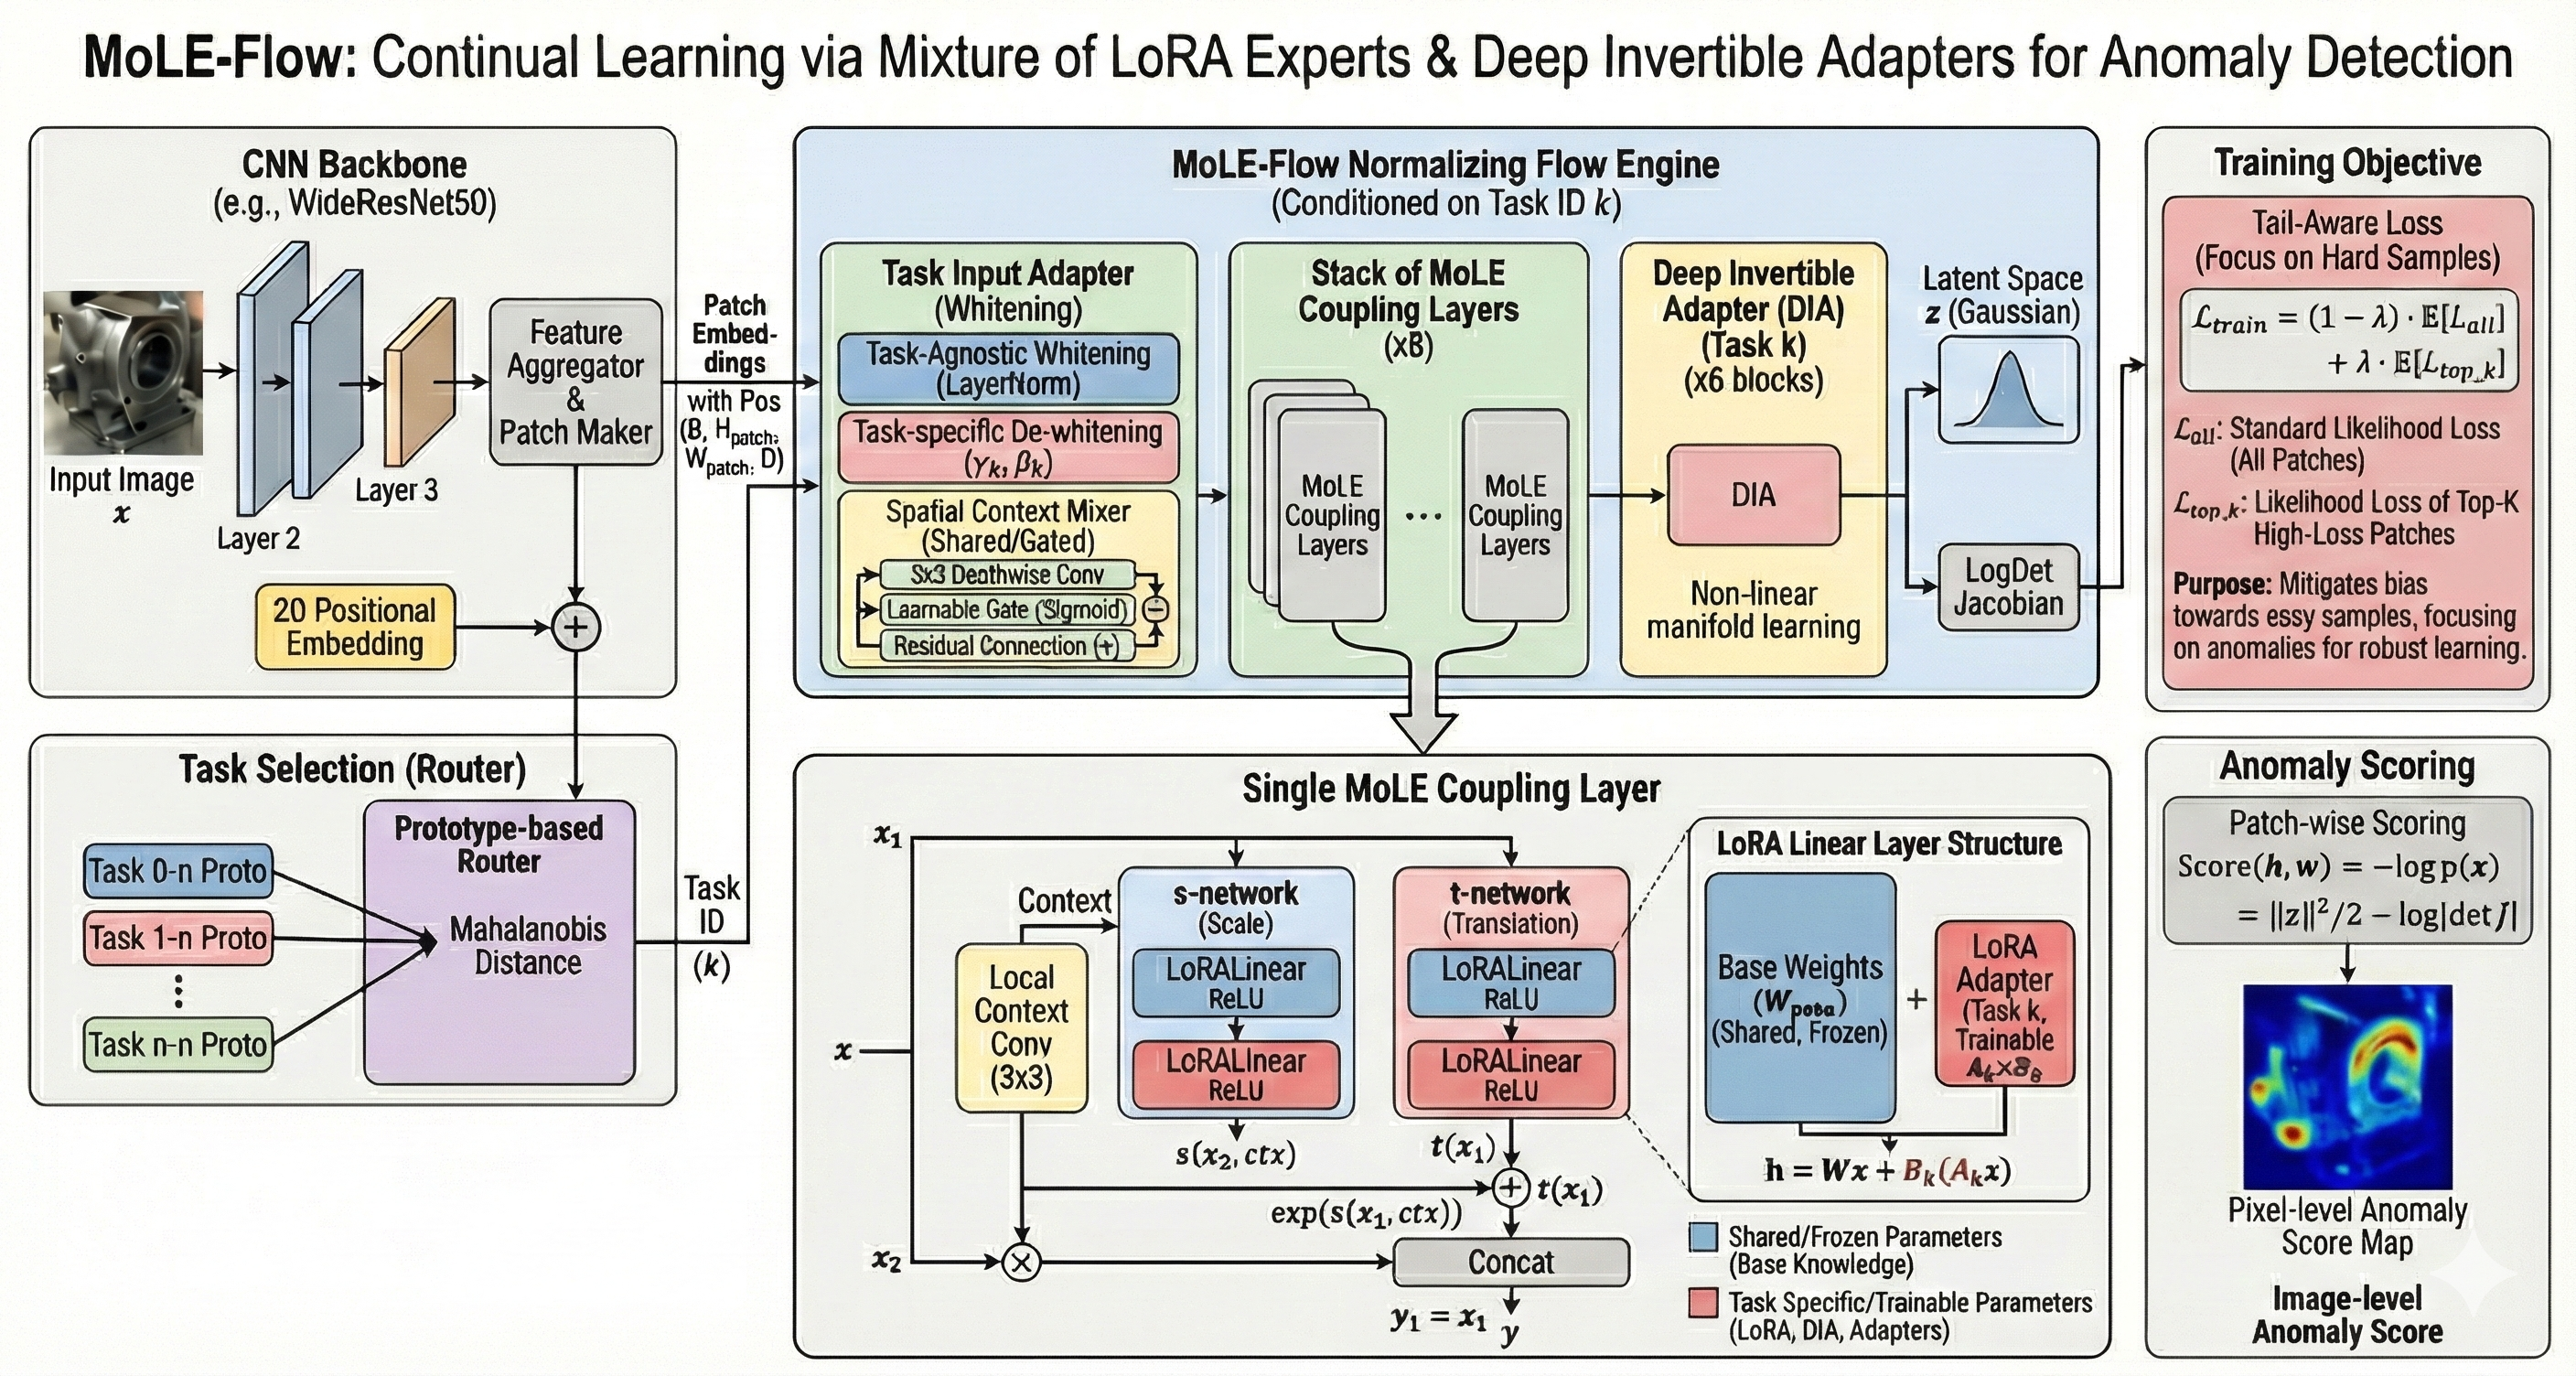
\includegraphics[width=\textwidth]{figures/main2.png}
    \caption{Overview of the proposed \textbf{MoLE-Flow} framework for continual anomaly detection on industrial images. Given sequential tasks, the base normalizing flow backbone is learned on the first task and then frozen. For each new task, only lightweight task-specific adapters (WhiteningAdapter, LoRA, DIA) are trained. At inference time, the prototype-based Mahalanobis router assigns each sample to the most relevant expert without requiring task ID.}
    \label{fig:main_figure}
\end{figure}

%=========================================================================================================
% 3.1 Key Insight: Why Parameter Decomposition Works for NF
%=========================================================================================================

\subsection{Key Insight: Parameter Decomposition for Continual Learning}
\label{sec:key_insight}

Before presenting our architecture, we establish the structural insight that motivates our approach. The isolation-efficiency dilemma admits only one logical resolution: \textbf{parameter decomposition} into shared and task-specific components.

\paragraph{The Only Solution: Parameter Decomposition.}
To achieve both parameter isolation (no inter-task interference) and parameter efficiency (no full model copies), we must decompose parameters as:
\begin{equation}
    \mathbf{W}_{\text{task}} = \mathbf{W}_{\text{shared}} + \Delta\mathbf{W}_{\text{task}},
\end{equation}
where $\mathbf{W}_{\text{shared}}$ is frozen after initial training and $\Delta\mathbf{W}_{\text{task}}$ is task-specific with $|\Delta\mathbf{W}| \ll |\mathbf{W}|$. This is the only strategy satisfying both constraints:

\begin{table}[h]
\centering
\small
\begin{tabular}{lccc}
\toprule
\textbf{Strategy} & \textbf{Isolation} & \textbf{Efficiency} & \textbf{Assessment} \\
\midrule
Full Model Copy & \checkmark & $\times$ ($O(N \cdot P)$) & Impractical \\
Shared Weights & $\times$ (interference) & \checkmark ($O(P)$) & Forgetting \\
\textbf{Decomposition} & \checkmark (delta only) & \checkmark ($O(P + N \cdot \delta)$) & \textbf{Both satisfied} \\
\bottomrule
\end{tabular}
\end{table}

\paragraph{Why Normalizing Flows Are Uniquely Suited.}
The critical question is: \emph{in which models can parameter decomposition be applied safely?} Not all generative models permit arbitrary internal reparameterization:

\begin{itemize}
    \item \textbf{VAE}: Encoder $q(z|x)$ and decoder $p(x|z)$ are jointly optimized via ELBO. Inserting adapters in only one component breaks latent space alignment, invalidating likelihood computation.

    \item \textbf{Diffusion Models}: The denoiser must maintain consistent behavior across all timesteps. Adapter effects accumulate unpredictably along sampling trajectories.

    \item \textbf{Normalizing Flows}: Coupling layers guarantee invertibility through their \emph{structure}, not their subnet implementation. The subnets $s(\cdot)$ and $t(\cdot)$ can be \emph{arbitrary functions}~\cite{dinh2017realnvp}---including decomposed functions---without affecting flow validity.
\end{itemize}

\begin{table}[h]
\centering
\small
\begin{tabular}{lcc}
\toprule
\textbf{Model} & \textbf{Effect of Decomposition} & \textbf{Theoretical Guarantees} \\
\midrule
VAE & Encoder-decoder misalignment & $\times$ Broken \\
Diffusion & Sampling trajectory distortion & $\times$ Broken \\
\textbf{NF Coupling} & \textbf{Subnet structure agnostic} & \checkmark \textbf{Preserved} \\
\bottomrule
\end{tabular}
\end{table}

This structural property---which we term the \emph{Arbitrary Function Property}---is the foundation of MoLE-Flow.

%=========================================================================================================
% 3.2 Design Principle 1
%=========================================================================================================

\subsection{Design Principle: Invertibility-Independence Decomposition}
\label{sec:design_principle}

\begin{principle}[Invertibility-Independence Decomposition]
In affine coupling layers, the invertibility guarantee depends solely on the coupling structure---the input splitting and affine transformation form---not on how the subnet functions $s(\cdot)$ and $t(\cdot)$ are internally parameterized. For:
\begin{equation}
    \mathbf{y}_1 = \mathbf{x}_1, \quad \mathbf{y}_2 = \mathbf{x}_2 \odot \exp(s(\mathbf{x}_1)) + t(\mathbf{x}_1),
\end{equation}
invertibility holds for any differentiable $s$ and $t$, with log-determinant $\log|\det J| = \sum_i s_i(\mathbf{x}_1)$ depending only on output values, not internal structure.
\end{principle}

\paragraph{Practical Consequence.} This principle enables decomposing subnets as:
\begin{equation}
    \text{MoLESubnet}(\mathbf{x}) = \text{MLPBase}(\mathbf{x}; \Theta_{\text{base}}) + \frac{\alpha}{r}\mathbf{B}_t(\mathbf{A}_t \mathbf{x}),
\end{equation}
where $\Theta_{\text{base}}$ is frozen after Task 0 and $\{\mathbf{A}_t, \mathbf{B}_t\}$ are task-specific low-rank adapters. This achieves $O(N \times \text{rank})$ scaling rather than $O(N \times \text{params})$, with complete parameter isolation by design.

\paragraph{Distinction from Prior Work.} This principle is not a claim that LoRA works universally---LoRA is well-established~\cite{hu2021lora}. Rather, it identifies a \emph{structural property of normalizing flows} that makes parameter isolation feasible by design, a property unavailable in VAEs or diffusion models where component modifications propagate unpredictably.

%=========================================================================================================
% 3.3 MoLE-Flow Architecture Overview
%=========================================================================================================

\subsection{MoLE-Flow Architecture}
\label{sec:architecture}

MoLE-Flow (Mixture of LoRA Experts for Normalizing Flow) instantiates the above design principle for continual anomaly detection. The framework comprises a feature extractor, MoLE-based normalizing flow, task-specific adapters, and a prototype-based router.

The core strategy for continual learning is \textbf{Parameter Isolation}: the backbone and base normalizing flow parameters are shared and frozen after Task 0, while task-specific adaptations are confined to lightweight adapters (LoRA, WhiteningAdapter, DIA). This achieves both memory efficiency and complete inter-task interference prevention.

The complete pipeline is:
\begin{enumerate}
\item Feature extraction and patch embedding generation from backbone
\item Positional encoding addition to patch embeddings
\item Distribution alignment via Whitening Adapter
\item Spatial context mixing for local neighborhood information
\item Probability distribution estimation via Normalizing Flow with LoRA
\item Likelihood-based anomaly scoring
\end{enumerate}

Formally:
\begin{equation}
\label{eq:pipeline}
\mathbf{x} \xrightarrow{\text{Backbone}} \mathbf{F} \xrightarrow{\text{PE}} \mathbf{F}' \xrightarrow{\text{Whitening}} \hat{\mathbf{F}} \xrightarrow{\text{SCM}} \tilde{\mathbf{F}} \xrightarrow{\text{NF+LoRA}} \mathbf{z}' \xrightarrow{\text{DIA}} (\mathbf{z}, \log|\det \mathbf{J}|)
\end{equation}

\paragraph{Notation.}
We denote $\mathbf{X} \in \mathbb{R}^{B \times H \times W \times D}$ as the patch embedding tensor with batch size $B$, spatial resolution $H \times W$, and feature dimension $D$.
$\mathbf{x}_{u,v} \in \mathbb{R}^D$ represents the individual patch vector at position $(u,v)$.
$t \in \{0, 1, \ldots, T-1\}$ is the task index, and $\mathbf{J}_f$ denotes the Jacobian matrix of function $f$.
$\lambda_{\text{tail}}$ is the weight for Tail-Aware Loss, and $\lambda_{\text{reg}}$ is the covariance regularization term.

During Task 0, both the base normalizing flow and task-specific components (LoRA, Whitening Adapter, DIA) are jointly trained. After Task 0 completion, the base parameters are frozen, and subsequent tasks train only task-specific adapters.

\subsection{Feature Extraction \& Preprocessing}
\label{sec:feature_extraction}

입력 이미지의 특징을 추출하고 각 작업별 전문가를 학습시키기 위한 입력으로 사용하기 위해 다음과 같은 전처리를 수행한다.

\subsubsection{Feature Extractor \& Patch Embedding}
\begin{itemize}
    \item 사전 학습된 Feature Extractor를 통해 특징을 추출한다.
    \item 이때 intermediate layer의 출력을 활용하여 다중 스케일 정보(multi-scale information)를 얻는다.
    \item PatchCore와 유사하게 입력 이미지의 지역적 특성을 추출한다.
    \item 추출된 특징 맵을 패치 단위로 분할한 뒤 풀링 과정을 거쳐 패치 임베딩을 생성한다.
    \item 최종적으로 $\mathbf{F} \in \mathbb{R}^{B \times H \times W \times D}$ 형태의 패치 임베딩을 얻으며, 여기서 $H \times W$는 패치 그리드 크기, $D$는 특징 차원이다.
\end{itemize}

\subsubsection{Positional Encoding}
\begin{itemize}
    \item Normalizing Flow는 permutation invariance 특성을 갖기 때문에, 2차원 구조가 아닌 patch embedding 각각이 독립적으로 처리된다.
    \item 각 패치의 공간적 위치 정보를 보존하기 위해 2D sinusoidal positional encoding $\mathbf{P}$를 패치 임베딩에 더한다.
    \item 수식으로 표현하면 다음과 같다:
\begin{equation}
\mathbf{F}' = \mathbf{F} + \mathbf{P}, \quad \mathbf{P} \in \mathbb{R}^{H \times W \times D}
\end{equation}
\end{itemize}

%=========================================================================================================
\subsection{Whitening Adapter}
%=========================================================================================================

\label{sec:adapters}
\begin{itemize}
\item MoLE-Flow는 첫 번째 작업 학습 이후 Base Flow의 파라미터를 동결(Freeze)
\item 이는 모델이 초기 학습 데이터의 분포 통계량에 피팅됨을 의미
\item 새로운 작업의 입력 분포가 이와 크게 다를 경우(Covariate Shift), 다음과 같은 문제 발생:
    \begin{itemize}
    \item 고정된 Base Network의 가중치는 최적의 활성화를 일으키지 못함
    \item 제한된 용량(Low-Rank)을 가진 LoRA가 전역적인 분포 차이까지 보정해야 하는 과도한 부담
    \item 학습 초기 수렴 지연 및 최적화 난이도 증가
    \end{itemize}
\item Whitening Adapter 도입을 통해 이를 해결하고자 함:
    \begin{itemize}
    \item 입력 데이터를 강제로 표준 정규 분포로 정렬(Alignment)
    \item 고정된 Base Flow가 항상 일관된 스케일의 입력을 처리하도록 보장
    \item LoRA가 분포 보정이 아닌 작업 고유의 미세 특징 학습에만 집중 가능
    \item 파라미터 분리 구조 하에서 학습 효율성과 안정성 극대화
    \end{itemize}
\end{itemize}

\textbf{Whitening Adapter는 Whitening과 De-whitening의 두 단계로 구성됨.}

\subsubsection{\textbf{Task-Agnostic Whitening}} 
\begin{itemize}
\item 입력 특징 $\mathbf{F}'$에 대해 학습 파라미터가 없는 LayerNorm 적용
\item 평균 0, 분산 1의 표준 정규 분포로 변환:
\begin{equation}
\mathbf{x}_{\text{white}} = \text{LayerNorm}(\mathbf{F}', \text{elementwise\_affine}=\text{False}) = \frac{\mathbf{F}' - \mathbb{E}[\mathbf{F}']}{\sqrt{\text{Var}[\mathbf{F}'] + \epsilon}}
\end{equation}
\item Task 0 이후 Base Flow는 동결되므로, 새로운 작업의 입력 분포가 달라지면 모델이 제대로 반응하지 못함
\item 새로운 작업의 데이터가 들어와도 강제 정규화를 통해 입력을 표준화하여 분포의 스케일 차이를 미리 제거
\item Normalizing Flow의 최적화 난이도를 낮추고 학습 안정성 확보
\item 모든 데이터를 표준 정규 분포로 정규화한 후, De-whitening을 통해 Base Flow의 최적 동작 범위 내로 재조정
\end{itemize}

\subsubsection{\textbf{Task-Specific De-whitening}} 
\begin{itemize}
\item Whitening으로 제거된 통계적 특성에 \textbf{해당 작업을 가장 잘 표현할 수 있는 최적의 통계적 특성을 다시 부여}
\item 단순 복원이 아닌, \textbf{고정된 Base Flow가 처리하기 가장 효율적인 형태로 데이터를 재조정(Recalibration)}
\item 정규화된 특징 $\mathbf{x}_{\text{white}}$에 대해 작업별 학습 가능한 파라미터 $\gamma_t$(스케일)와 $\beta_t$(이동)를 적용한 아핀 변환:
\begin{align}
\gamma_t &= 0.5 + 1.5 \cdot \sigma(\gamma_{\text{raw}}) \\
\beta_t &= 2.0 \cdot \tanh(\beta_{\text{raw}}) \\
\hat{\mathbf{F}}_t &= \gamma_t \odot \mathbf{x}_{\text{white}} + \beta_t
\end{align}
여기서 $\sigma(\cdot)$는 시그모이드 함수

\item De-whitening 단계에서 작업별 학습 파라미터를 통해 각 작업의 고유한 특성을 복원
\item 단순한 원래 분포의 복원이 아니라, \textbf{고정된 모델의 매니폴드(Manifold) 상에서 각 작업 데이터가 가장 잘 표현될 수 있도록 최적의 통계적 위치를 학습하는 과정}
\item 모든 작업에서 모든 특징 채널이 동등하게 중요한 것은 아니므로, $\gamma_t$는 채널별로 특징의 중요도를 조절:
    \begin{itemize}
    \item $\gamma_t$ 값 증가 $\rightarrow$ 해당 특징 증폭, Flow 모델이 더 민감하게 반응
    \item $\gamma_t$ 값 감소 $\rightarrow$ 해당 특징 억제, 노이즈로 간주
    \item 예시: '가죽' 작업에서는 미세한 질감(Texture) 채널의 $\gamma_t$ 증가, '나사' 작업에서는 전체적인 형태(Shape) 채널의 $\gamma_t$ 증가
    \end{itemize}
\end{itemize}

\paragraph{아핀 변환을 사용하는 이유:}
De-whitening에서 아핀 변환(Affine Transformation, $\mathbf{y} = \gamma \odot \mathbf{x} + \beta$)을 사용하는 이유는 \textbf{통계적 특성(평균, 분산)만 정확하게 조절하고, 데이터가 가진 본질적인 구조(Shape/Pattern)는 훼손하지 않기 위해서}이다.

\begin{itemize}
\item \textbf{통계적 정합성 (Statistical Consistency):} 
    \begin{itemize}
    \item 정규 분포를 다른 정규 분포로 변환하는 가장 자연스러운 방법은 아핀 변환이다.
    \item Whitening은 데이터를 표준 정규 분포 $\mathcal{N}(0, 1)$로 만들고, De-whitening은 이를 작업별 고유 분포 $\mathcal{N}(\mu_t, \sigma_t^2)$로 이동시킨다.
    \item 비선형 변환(예: $x^2$, $\exp(x)$)을 사용하면 분포의 모양 자체가 왜곡되어 정규 분포의 성질(Bell curve)을 잃어버리며, 이는 가우시안 기반 Normalizing Flow의 처리를 어렵게 만든다.
    \end{itemize}

\item \textbf{구조 보존 (Structure Preservation):}
    \begin{itemize}
    \item 아핀 변환은 공간을 늘리거나(Scale), 이동(Shift)만 하므로 \textbf{직선은 직선으로 남고, 평행선은 평행하게 유지}된다.
    \item 이미지 패치 내부의 픽셀 관계는 물체의 형상을 나타내므로, 아핀 변환은 이미지가 조금 밝아지거나 대비가 강해질 뿐 "고양이"가 "강아지"처럼 보이게 모양이 바뀌지 않는다.
    \item 반면 비선형 변환은 공간을 구부리거나 비틀어 직선이 곡선이 되고 모양이 뒤틀리므로, \textbf{데이터의 내용(Content) 자체를 변질}시킬 위험이 있다.
    \item Adapter의 역할은 "입력의 톤(Tone)을 맞추는 것"이지, "내용을 재창조하는 것"이 아니므로 형태를 보존하는 아핀 변환이 최적이다.
    \end{itemize}

\item \textbf{역할 분담 (Division of Labor):}
    \begin{itemize}
    \item MoLE-Flow 전체 구조에서 Adapter는 서로 다른 도메인(가죽, 나사)의 \textbf{시작점(Start Point)을 맞춰주는 역할}로, 가장 기초적인 1차 모멘트(평균)와 2차 모멘트(분산)만 빠르고 정확하게 맞추면 된다.
    \item 실제 데이터의 복잡하고 비선형적인 분포 모델링은 Base Flow와 LoRA가 담당한다.
    \item Adapter가 굳이 복잡한 비선형 변환을 수행하여 연산량을 늘리고 최적화를 어렵게 만들 필요가 없으며, 이는 Batch Normalization~\cite{ioffe2015batchnorm}이 학습 가능한 파라미터 $\gamma$, $\beta$를 두어 표현력을 복원하는 원리와 동일하다.
    \item 또한, 본 접근법은 FiLM(Feature-wise Linear Modulation)~\cite{perez2018film}의 조건부 아핀 변환과 개념적으로 연결되며, 이를 지속 학습 환경의 도메인 적응에 특화시킨 것으로 볼 수 있다.
    \end{itemize}
\end{itemize}

결론적으로, Affine transformation은 \textbf{데이터의 본질은 건드리지 않으면서, 모델이 편식하지 않게 통계적 특성만 맞춰주는 가장 안전하고 효율적인 방법}이다.

\noindent 결과적으로 Whitening Adapter는:
\begin{itemize}
\item Whitening을 통해 불필요한 분포 격차를 제거
\item De-whitening을 통해 필요한 작업 고유의 특성을 학습된 형태로 복원
\item 입력 데이터의 글로벌한 표준화와 작업별 최적화를 동시에 달성
\item Base Flow는 Task 0의 데이터 분포에 최적화되어 고정되어 있으므로, 새로운 작업의 데이터가 "Task 0의 매니폴드 영역"과 동떨어져 있으면 Base Flow의 활성 함수들이 제대로 작동하지 않음
\item De-whitening은 $\gamma_t$와 $\beta_t$를 조절하여 정규화된 데이터를 Base Flow가 학습했던 익숙한 영역 근처로 매핑하고, 새로운 데이터가 Base Flow의 활성 함수들이 가장 잘 작동하는 구간(Active Region)에 위치하도록 보장
\item 고정된 Base Flow의 효과적인 재활용을 가능하게 하며, 지속 학습 환경에서 안정적이고 효율적인 학습을 보장
\end{itemize}

%=========================================================================================================
\subsection{\textbf{Spatial Context Mixer}}
%=========================================================================================================
\label{sec:spatial_mixer}
\begin{itemize}
    \item Normalizing Flow는 입력으로 이미지로 부터 생성된 각 Patch embedding들을 독립적으로 처리하여 우도를 계산하고 이를 통해 분포를 학습한다.    
\end{itemize}
\begin{equation}
    p(\mathbf{X}) \approx \prod_{u=1}^{H} \prod_{v=1}^{W} p(\mathbf{x}_{u,v})
\end{equation}
\begin{itemize}
    \item 이러한 Normalizing Flow의 구조상 위치 $(u, v)$의 특징 벡터 $\mathbf{x}_{u,v}$를 인접한 이웃들과 독립적(Independent and Identically Distributed, i.i.d.)으로 처리한다.
    \item 이러한 독립적 처리는 \textbf{구조적 사각지대(Structural Blind Spot)}를 야기한다.
    \begin{itemize}
        \item \textbf{공간적 상관관계의 누락:} 긁힘(Scratch)이나 얼룩(Stain)과 같은 미세 결함은 단일 패치 내부의 값보다는 주변 패치와의 \textbf{불연속성(Discontinuity)}으로 정의된다. 그러나 Normalizing Flow는 패치를 독립적으로 처리하므로 이러한 국소적 대조(Local Contrast)를 인지하지 못한다.
        \item \textbf{문맥 정보의 부재:} 정상 데이터의 분포는 주변 문맥에 따라 달라질 수 있다. 독립적인 처리는 $p(\mathbf{x}_{u,v} | \text{Neighbors})$와 같은 조건부 확률을 모델링할 수 없다.
    \end{itemize}
\end{itemize}

\paragraph{\textbf{Mechanism: Gated Depthwise Aggregation}}
\begin{itemize}
    \item 이러한 한계를 극복하기 위해 Normalizing Flow 입력 직전에 \textbf{Spatial Context Mixer}를 도입
    \item 이 모듈은 파라미터 효율성을 극대화하면서, 각 패치가 주변 정보를 물리적으로 집계할 수 있도록 설계
\end{itemize}

\begin{itemize}
    \item \textbf{Spatial Aggregation (Depthwise Convolution):}
    \begin{itemize}
        \item Mixer는 채널 간의 간섭 없이 오직 공간적 정보만을 통합하기 위해 \textbf{Depthwise Convolution}~\cite{howard2017mobilenets}을 사용한다.
        \begin{equation}
            \mathbf{C}^{(c)}_{u,v} = \sum_{i=-\lfloor K/2 \rfloor}^{\lfloor K/2 \rfloor} \sum_{j=-\lfloor K/2 \rfloor}^{\lfloor K/2 \rfloor} \mathbf{W}^{(c)}_{i,j} \cdot \mathbf{x}^{(c)}_{u+i, v+j}
        \end{equation}
        \item 여기서 $K$는 커널 크기(홀수, 기본값 3), $c$는 채널 인덱스, $\mathbf{x}^{(c)}$는 $c$번째 채널의 입력 특징 맵, $\mathbf{W}^{(c)} \in \mathbb{R}^{K \times K}$는 해당 채널의 커널 가중치, $\mathbf{C}$는 추출된 문맥 특징(Context Feature)이다.
        \item 이를 통해 각 특징 벡터는 자신의 위치뿐만 아니라 주변 이웃의 정보를 집계한다.
    \end{itemize}
\end{itemize}

\begin{itemize}
    \item \textbf{Adaptive Interpolation (Learnable Gating):}
    \begin{itemize}
        \item 단순한 잔차 연결(Residual Addition) 대신, 모델은 원본 정보와 문맥 정보의 반영 비율을 스스로 결정하는 \textbf{적응형 보간(Adaptive Interpolation)} 메커니즘을 사용한다.
        \begin{equation}
            \alpha = \sigma(\theta_{\text{gate}})
        \end{equation}
        \begin{equation}
            \mathbf{z}_{u,v} = (1 - \alpha) \cdot \mathbf{x}_{u,v} + \alpha \cdot \mathbf{C}_{u,v}
        \end{equation}
        \item 여기서 $\sigma(\cdot)$는 시그모이드(Sigmoid) 함수이며, $\theta_{\text{gate}}$는 학습 가능한 스칼라 파라미터이다.
        \item 이러한 게이팅 구조는 학습 초기($\alpha \approx 0.5$ 또는 초기화에 따라 조절)에 원본 특징과 문맥 특징을 균형 있게 학습하다가, 최적화 과정에서 태스크에 따라 공간 정보의 중요도($\alpha$)를 동적으로 조절할 수 있게 한다.
        \item 예를 들어, 텍스처가 균일한 표면(가죽 등)에서는 $\alpha$를 높여 주변 정보를 적극 활용하고, 복잡한 객체에서는 조절하는 식이다.
    \end{itemize}
\end{itemize}

\begin{itemize}
    \item \textbf{Effect: Pseudo-Dependency Modeling}
    \begin{itemize}
        \item 최종적으로 생성된 특징 벡터 $\mathbf{z}_{u,v}$는 Normalizing Flow에 독립적인 개체로 입력되지만, 정보적으로는 이미 주변 이웃의 상태 $\mathcal{N}_{u,v}$를 내포하고 있다.
        \begin{equation}
            \mathbf{z}_{u,v} \approx \text{Encode}(\mathbf{x}_{u,v} \oplus \mathcal{N}_{u,v})
        \end{equation}
        \item 결과적으로 Normalizing Flow는 구조 변경 없이도 $\mathbf{z}_{u,v}$를 통해 간접적으로 조건부 확률 $p(\mathbf{x}_{u,v} | \mathcal{N}_{u,v})$을 학습하는 효과(Pseudo-Dependency)를 얻게 되며, 이는 구조적 이상 탐지 성능을 비약적으로 향상시킨다.
    \end{itemize}
\end{itemize}

%=========================================================================================================
\subsection{\textbf{MoLE-Flow Architecture}}
\label{sec:moleflow}
%=========================================================================================================
\begin{itemize}
    \item{MoLE-Flow는 Feature Extractor로부터 추출된 패치 임베딩을 잠재 공간(Latent Space)의 가우시안 분포로 매핑하여 정상 데이터의 확률 밀도를 추정하는 생성 모델.}
    \item{본 모델은 RealNVP~\cite{dinh2016realnvp} 기반의 가역적 구조를 따르며, 연속 학습 환경에서 파멸적 망각을 방지하고 이상 탐지 성능을 극대화하기 위해 다음과 같은 핵심 요소들로 구성된다.}
\end{itemize}

\begin{itemize}
    \item \textbf{MoLEContextSubnet}: 
    \begin{itemize}
        \item Coupling Layer 내부에서 변환 파라미터(Scale, Shift)를 생성하는 핵심 모듈이다.
        \item 단순한 MLP 대신 공간적 문맥(Spatial Context)을 고려하도록 설계되어, 이상 탐지의 핵심인 `국소적 대조(Local Contrast)' 정보를 스케일링 변환에 반영한다.
        \item Base weight를 Task 0에서만 학습 후 freeze 함으로써 anchor로 활용하며, LoRA Adapter를 활용해 작업별 분포 차이(Distribution Shift)를 저비용으로 학습한다.         
    \end{itemize}
    \item \textbf{Deep Invertible Adapter (DIA)}:
    \begin{itemize}
        \item NF의 출력단에 위치하여 선형 LoRA가 표현하기 어려운 작업 특화 비선형 매니폴드를 학습하는 가역적 어댑터
        \item 완전히 독립적인 작업별 파라미터를 사용하여 작업 간 간섭 없이 정밀한 분포 보정 수행
        \item Affine Coupling Block 구조를 사용하여 가역성을 보장하고 정확한 log-determinant 계산 가능
    \end{itemize}
\end{itemize}

\subsubsection{\textbf{MoLEContextSubnet: Context-Aware \& Task-Adaptive Design}}
\label{sec:molesubnet}

\begin{itemize}
    \item MoLEContextSubnet은 Normalizing Flow의 각 Coupling Layer 내부에서 변환 파라미터 $(\mathbf{s}, \mathbf{t})$를 생성하는 핵심 모듈이다.
    \item 일반적인 Coupling Layer가 단순한 MLP로 파라미터를 예측하는 것과 달리, 본 모듈은 \textbf{공간적 문맥 인지(Spatial Context Awareness)}와 \textbf{작업 적응성(Task Adaptivity)}을 동시에 갖추도록 설계되었다.
    \item 본 모듈은 3x3 Depthwise Convolution을 통해 공간적 문맥을 추출하고, 이를 통해 주변 이웃과의 대조 정보를 포착하여 이상 탐지에 효과적으로 활용한다.
    \item 스케일과 이동 예측에 비대칭적인 네트워크를 구성하여 서로 다른 입력을 사용하여 서로 다른 특성을 포착하도록 설계되었다.
    \item MoLEContextSubnet은 크게 세 부분으로 구성된다: (1) Spatial Context Conditioning, (2) Context-Aware s-network, (3) Context-Free t-network.        
\end{itemize}

\begin{itemize}
    \item \textbf{Spatial Structure Recovery \& Context Extraction:}:
    \begin{itemize}
        \item 일반적인 Normalizing Flow는 입력을 1차원 벡터로 평탄화하여 처리하므로 패치 간 공간적 인접성 정보가 소실된다.
        \item 이를 보완하기 위해 MoLEContextSubnet은 입력을 2차원 이미지 형태로 재구성하여 공간 구조를 복원한 후, $3 \times 3$ Depthwise Convolution으로 지역적 문맥 $\mathbf{c}(\mathbf{x})$를 추출한다.
        \item 추출된 문맥은 학습 가능한 게이팅을 통해 반영 비율이 조절된다:
        \begin{equation}
            \mathbf{ctx} = \alpha \cdot \mathbf{c}(\mathbf{x}), \quad \text{where } \alpha = \alpha_{\max} \cdot \sigma(\theta_{\text{scale}})
        \end{equation}
    \end{itemize}
\end{itemize}

\begin{itemize}
    \item \textbf{Context-Aware s-network}:
    \begin{itemize}
        \item 이상 탐지에서 결함은 주로 주변과의 \textbf{불연속성(Contrast)}으로 나타난다.
        \item 스케일 파라미터는 이러한 국소적 대비를 포착해야 하므로, 원본 특징과 문맥을 결합하여 입력으로 사용한다:
        \begin{equation}
            \mathbf{s} = \text{Linear}_2^{(s)}(\text{ReLU}(\text{Linear}_1^{(s)}([\mathbf{x}; \mathbf{ctx}])))
        \end{equation}       
    \end{itemize}
    \item \textbf{Context-Free t-network}:
    \begin{itemize}
        \item 분포의 위치 이동(Shift)은 패치 고유의 특성에 종속되므로, 문맥 없이 원본 특징만으로 예측한다:
        \begin{equation}
            \mathbf{t} = \text{Linear}_2^{(t)}(\text{ReLU}(\text{Linear}_1^{(t)}(\mathbf{x})))
        \end{equation}
    \end{itemize}
    \item 위 수식의 각 $\text{Linear}$ 레이어는 LoRALinear로 구현된다.
    \item LoRALinear는 Base 출력에 작업별 LoRA 출력을 더하는 구조로, 다음과 같이 계산된다:
    \begin{equation}
        \mathbf{h}(\mathbf{x}) = \underbrace{\mathbf{W}_{\text{base}}\mathbf{x} + \mathbf{b}_{\text{base}}}_{\text{Base (frozen after Task 0)}} + \underbrace{\frac{\alpha}{r}(\mathbf{B}_t\mathbf{A}_t)\mathbf{x} + \mathbf{b}_t}_{\text{Task-specific LoRA}}
    \end{equation}
    \item Task 0 학습 후 $\mathbf{W}_{\text{base}}$와 $\mathbf{b}_{\text{base}}$는 동결되어, 이후 작업 학습 시 수정되지 않는다.
    \item 새로운 작업은 독립적인 LoRA 행렬 $(\mathbf{A}_t, \mathbf{B}_t)$과 task bias $\mathbf{b}_t$만 학습하므로, 기존 작업의 변환 능력이 보존되어 파멸적 망각이 방지된다.
    \item 추론 시에는 Router가 예측한 작업의 LoRA만 활성화되므로 작업 간 간섭이 발생하지 않는다.
\end{itemize}

\paragraph{가역성 보장.}
LoRA가 Normalizing Flow의 가역성에 영향을 미치는지에 대해 명확히 할 필요가 있다.
Affine Coupling Layer에서 가역성은 변환 구조 자체(입력 분할 및 아핀 변환)에 의해 보장되며, scale과 shift 파라미터를 생성하는 subnet의 구조에는 의존하지 않는다.
즉, subnet이 MLP이든, LoRA가 적용된 네트워크이든 관계없이 다음이 성립한다:
\begin{equation}
    \mathbf{y} = [\mathbf{x}_1, \mathbf{x}_2 \odot \exp(\mathbf{s}) + \mathbf{t}] \quad \Leftrightarrow \quad \mathbf{x} = [\mathbf{y}_1, (\mathbf{y}_2 - \mathbf{t}) \odot \exp(-\mathbf{s})]
\end{equation}
LoRA는 subnet 내부의 선형 레이어에만 적용되며, 이는 Jacobian 계산에 직접 관여하지 않는다.
따라서 LoRA 적용 여부와 무관하게 전체 Normalizing Flow의 가역성과 정확한 likelihood 계산이 보장된다.

\begin{itemize}
    \item \textbf{Spatial Context Mixer와의 관계: 계층적 문맥 처리}:
    \begin{itemize}
        \item Section~\ref{sec:spatial_mixer}의 Spatial Context Mixer와 MoLEContextSubnet 내부의 Context Conditioning은 모두 공간적 문맥을 활용하지만, 그 역할이 명확히 구분된다.
        \item Spatial Context Mixer는 Flow 입력 이전에 ``이 패치가 어떤 이웃을 가지는가''를 특징 자체에 인코딩하는 \textbf{전처리} 모듈이다.
        \item MoLEContextSubnet의 Context Conditioning은 각 Coupling Layer 내부에서 ``이 이웃 관계에서 어떤 스케일 변화가 적절한가''를 결정하는 \textbf{변환 가이드} 역할을 한다.
        \item 두 모듈이 모두 필요한 이유는 \textbf{계층적 문맥 처리(Hierarchical Context Processing)} 관점에서 이해할 수 있다:
        \item 입력 수준의 문맥 인코딩(Spatial Context Mixer)과 변환 수준의 적응적 스케일링(MoLEContextSubnet)은 상호 보완적으로 작용하여, 단일 모듈만으로는 달성하기 어려운 정교한 이상 탐지 성능을 가능하게 한다.
    \end{itemize}
\end{itemize}


\subsubsection{Deep Invertible Adapter (DIA)}
\label{sec:dia}
\begin{itemize}
    \item DIA는 Normalizing Flow 출력단에 위치하며, MoLEContextSubnet이 처리하지 못한 작업 특화 비선형 매니폴드를 정밀 보정한다.
    \item Affine Coupling Block으로 구성되며, 각 작업별로 독립적인 파라미터가 분리되어 있다.
    \item 수학적으로, 전체 변환과 밀도 추정은 다음과 같이 표현된다:
    \begin{equation}
        \mathbf{z}_{\text{final}} = f_{\text{DIA}}^{(t)}(\mathbf{z}_{\text{base}}), \quad \log p(\mathbf{x}) = \log p(\mathbf{z}_{\text{final}}) + \log|\det \mathbf{J}_{\text{base}}| + \log|\det \mathbf{J}_{\text{DIA}}|
    \end{equation}
    \item 각 AffineCouplingBlock의 변환:
    \begin{align}
        [\mathbf{x}_1, \mathbf{x}_2] &= \text{Split}(\mathbf{x}) \\
        \mathbf{s}, \mathbf{t} &= \text{SimpleSubnet}(\mathbf{x}_1) \\
        \mathbf{y}_2 &= \mathbf{x}_2 \odot \exp(\alpha_{\text{clamp}} \cdot \tanh(\mathbf{s}/\alpha_{\text{clamp}})) + \mathbf{t} \\
        \mathbf{y} &= \text{Concat}(\mathbf{x}_1, \mathbf{y}_2)
    \end{align}
\end{itemize}


\begin{itemize}
    \item \textbf{DIA의 핵심 장점}:
    \begin{itemize}
        \item \textbf{비선형 매니폴드 적응}: 선형 LoRA가 표현할 수 없는 복잡한 분포 변환을 학습한다.
        \item \textbf{가역성 보장}: 정규화 흐름의 밀도 추정 속성이 유지되므로, 이상 점수의 확률적 해석이 보존된다.
        \item \textbf{완전한 작업 분리}: 작업별로 완전히 독립적인 파라미터를 사용하여 작업 간 간섭이 없다.
        \item \textbf{후처리 위치}: 기반 NF의 뒷단에 위치하여, 기반 NF가 학습한 범용 변환을 먼저 적용하고 DIA가 작업 특화 조정을 수행한다.
    \end{itemize}
\end{itemize}

\begin{itemize}
    \item \textbf{MoLEContextSubnet과의 차이}:
    \begin{itemize}
        \item MoLEContextSubnet과 DIA는 모두 Affine Coupling 구조를 기반으로 하지만, 서로 다른 설계 철학을 따른다.
        \item \textbf{MoLEContextSubnet}은 ``\textit{공간 인지형 범용 변환기(Spatially-Aware Universal Transformer)}''로서, 고정된 Base weights를 anchor로 삼아 범용 변환 능력을 보존하면서 LoRA를 통해 작업별 적응을 수행한다.
        \item Spatial context conditioning을 통해 국소적 이상 패턴에 민감하게 반응하며, 모든 작업에서 공유되는 ``정상 $\rightarrow$ 표준 정규분포'' 변환의 뼈대를 제공한다.
        \item 반면 \textbf{DIA}는 ``\textit{작업 특화 분포 보정기(Task-Specific Distribution Corrector)}''로서, 작업별로 완전히 독립적인 파라미터를 사용하여 작업 고유의 분포를 정밀 보정한다.
        \item DIA가 spatial context를 사용하지 않는 이유는 세 가지다:
        \begin{itemize}
            \item (1) DIA는 잠재 공간에서 동작하며, 이 시점에서 공간 정보는 이미 MoLEContextSubnet을 통해 인코딩되어 있다.
            \item (2) MoLEContextSubnet이 ``공간 인지 변환''을, DIA가 ``분포 정밀 보정''을 담당하는 명확한 역할 분리가 효율적이다.
            \item (3) 작업별 독립 파라미터를 사용하는 DIA에 추가 context 모듈은 파라미터 오버헤드를 증가시킨다.
        \end{itemize}
    \end{itemize}
\end{itemize}

\subsection{\textbf{Training Objective}}
\label{sec:training_objective}

\begin{itemize}
    \item 모델의 학습과 이상 탐지는 입력 데이터가 잠재 공간의 정규 분포로 얼마나 잘 매핑되는지를 측정하는 Log-likelihood 계산을 통해 이루어진다.
    \item 이 과정은 크게 Forward 변환 및 Jacobian 누적, 잠재 확률 계산, 그리고 최종 likelihood 산출을 통해 이루어진다.
\end{itemize}

\subsubsection{\textbf{Likelihood Calculation}}

\begin{itemize}
    \item 사전 학습된 특징 추출기로부터 생성된 입력 패치 임베딩은 잠재 변수 $\mathbf{z}$로 변환되며, 각 변환 단계의 부피 변화율인 log-determinant of Jacobian이 누적된다.    
    \item 입력 $\mathbf{x}$는 Task Adapter, Spatial Mixer, MoLEContextSubnet, DIA를 순차적으로 통과하며 최종 잠재 벡터 $\mathbf{z}$로 변환된다.    
    \item Flow와 DIA를 거치는 동안 발생된 log determinant Jacobian 값들이 합산된다:
        \begin{equation}
            \log|\det \mathbf{J}_{\text{total}}| = \log|\det \mathbf{J}_{\text{flow}}| + \log|\det \mathbf{J}_{\text{DIA}}|
        \end{equation}
        
    \item \textbf{Log-Determinant 계산:}
        \begin{itemize}
            \item MoLEContextSubnet과 DIA 모두 Affine Coupling 구조를 사용하며, 동일한 방식으로 log-determinant를 계산한다.
            \item 각 Affine Coupling Block은 입력을 두 부분 $\mathbf{x}_1, \mathbf{x}_2$로 분할하고, scale과 translation 파라미터를 생성한다.
            \item 수치 안정성을 위해 soft-clamping이 적용된 변환을 수행한다:
            \begin{equation}
                \mathbf{y}_1 = \mathbf{x}_1, \quad \mathbf{y}_2 = \mathbf{x}_2 \odot \exp(\tilde{\mathbf{s}}) + \mathbf{t}, \quad \text{where } \tilde{\mathbf{s}} = \alpha_{\text{clamp}} \cdot \tanh(\mathbf{s}/\alpha_{\text{clamp}})
            \end{equation}
            \item 이 변환의 Jacobian은 블록 하삼각 행렬 형태를 가지므로, log-determinant는 clamped scale 파라미터의 합으로 계산된다:
            \begin{equation}
                \log|\det \mathbf{J}_{\text{layer}}| = \sum_{i=1}^{D/2} \tilde{s}_i = \sum_{i=1}^{D/2} \alpha_{\text{clamp}} \cdot \tanh(s_i/\alpha_{\text{clamp}})
            \end{equation}
            \item MoLEContextSubnet의 $M$개 블록과 DIA의 $N$개 블록의 log-determinant가 각각 누적되어:
            \begin{equation}
                \log|\det \mathbf{J}_{\text{flow}}| = \sum_{k=1}^{M} \log|\det \mathbf{J}_{\text{layer}_k}|, \quad
                \log|\det \mathbf{J}_{\text{DIA}}| = \sum_{j=1}^{N} \log|\det \mathbf{J}_{\text{block}_j}|
            \end{equation}
            \item 최종적으로 두 값이 합산되어 전체 변환의 부피 변화율을 나타낸다.
        \end{itemize}
        
    \item \textbf{잠재 확률 계산}: 
    \begin{itemize}
        \item 잠재 변수 $\mathbf{z}_{\text{final}}$이 표준 정규분포를 따른다고 가정하고, 각 패치 위치에서의 log probability density를 계산한다.
    \begin{equation}
            \log p(\mathbf{z}_{\text{final}}) = -\frac{1}{2}\|\mathbf{z}_{\text{final}}\|_2^2 - \frac{D}{2}\log(2\pi)
        \end{equation}
    \end{itemize}
    \item \textbf{최종 likelihood 산출}: 변수 변환 공식에 따라 입력 공간에서의 log likelihood를 계산한다.
    \begin{equation}
        \log p(\mathbf{x}) = \log p(\mathbf{z}_{\text{final}}) + \log|\det \mathbf{J}_{\text{total}}|
    \end{equation}
\end{itemize}

\subsubsection{\textbf{Tail-Aware Loss}}

\begin{itemize}
    \item 일반적인 NF의 학습 방식을 따르는 경우 이미지 내 모든 패치의 우도 평균을 최대화하게 된다.
    \item 이는 모델이 대다수의 학습하기 ``쉬운'' 정상 패치에만 집중하게 되고, 분포의 꼬리(Tail)에 위치한 ``어려운'' 패치나 이상 징후를 간과하게 만드는 원인이 된다.
    \item 따라서 본 모델은 학습 시 Tail-Aware Loss를 도입하여, 전체 평균뿐만 아니라 손실 값이 높은 상위 $K\%$ 패치에 가중치를 두어 학습하도록 한다:
    \begin{equation}
        \mathcal{L}_{\text{train}} = (1 - \lambda_{\text{tail}}) \cdot \mathbb{E}[\mathcal{L}_{\text{all}}] + \lambda_{\text{tail}} \cdot \mathbb{E}[\mathcal{L}_{\text{top-k}}]
    \end{equation}
    \item 여기서 $\lambda_{\text{tail}} = 0.7$, $\mathcal{L}_{\text{top-k}}$는 상위 $K\%$ 고손실 패치의 평균 NLL이다.
    \item 이는 모델이 정상 분포의 경계(Boundary)를 더 명확하게 학습하도록 유도한다.
\end{itemize}

\subsection{\textbf{Task Routing \& Adapter Activation}}
\label{sec:task_routing}

\begin{itemize}
    \item Class-Incremental Learning (CIL) 환경에서는 추론 시 입력 이미지가 어느 task에 속하는지 사전 정보가 주어지지 않는다.
    \item 예를 들어, Task 0에서 \{bottle, cable, capsule\}을 학습하고 Task 1에서 \{carpet, grid\}를 학습한 경우, 추론 시 입력 이미지가 어느 task의 클래스인지 알 수 없다.
    \item 따라서 모델은 입력 이미지를 보고 자동으로 적절한 task를 선택하고, 해당 task의 adapters (LoRA, Input Adapter, DIA)를 활성화해야 한다.
    \item 이는 CIL의 핵심 과제로, 잘못된 task 선택은 부적절한 파라미터 활성화로 이어져 이상 탐지 성능을 크게 저하시킨다.
\end{itemize}

\subsubsection{\textbf{Prototype-Based Task Routing}}

\begin{itemize}
    \item Mahalanobis 거리 기반 Prototype Router~\cite{lee2018mahalanobis}를 사용하여 task를 자동으로 인식한다.
    
    \item \textbf{Prototype 구축 (Training Phase):}
    \begin{itemize}
        \item 각 task $t$의 학습 과정에서, 정상 샘플들의 특징 벡터를 수집하여 task-specific prototype을 구축한다.                    
        \item Prototype은 평균 벡터 $\boldsymbol{\mu}_t \in \mathbb{R}^D$와 공분산 행렬 $\boldsymbol{\Sigma}_t \in \mathbb{R}^{D \times D}$로 구성된다:
        \begin{align}
            \boldsymbol{\mu}_t &= \frac{1}{N_t} \sum_{i=1}^{N_t} \mathbf{f}_i^{(t)} \\
            \boldsymbol{\Sigma}_t &= \frac{1}{N_t - 1} \sum_{i=1}^{N_t} (\mathbf{f}_i^{(t)} - \boldsymbol{\mu}_t)(\mathbf{f}_i^{(t)} - \boldsymbol{\mu}_t)^\top + \lambda_{\text{reg}} \mathbf{I}
        \end{align}

        \item 여기서 $\mathbf{f}_i^{(t)}$는 Backbone의 가장 마지막 layer의 출력 feature vector $\mathbf{f}_{\text{backbone}} \in \mathbb{R}^D$를 이미지 레벨 특징 벡터로 사용한다.
        \item $N_t$는 task $t$의 학습 샘플 수, $\lambda_{\text{reg}}$는 수치 안정성을 위한 정규화 항($=10^{-5}$)이다.
        \item 공분산의 역행렬인 precision matrix $\boldsymbol{\Sigma}_t^{-1}$을 미리 계산하여 저장한다.
    \end{itemize}
    
    \item \textbf{Task Selection (Inference Phase):}
    \begin{itemize}
        \item 추론 시 입력 이미지 $\mathbf{x}_{\text{img}}$로부터 Backbone의 가장 마지막 layer의 출력 feature vector $\mathbf{f}_{\text{backbone}} \in \mathbb{R}^D$를 이미지 레벨 특징 벡터로 사용한다.
        \item 모든 학습된 task의 prototype과의 Mahalanobis 거리를 계산한다.
        \item Mahalanobis 거리는 단순 Euclidean 거리와 달리 각 task의 특징 분포의 형태(공분산)를 고려하므로, 분포 간 중첩이 있어도 더 정확한 task 구분이 가능하다.
        \item 가장 가까운 prototype을 가진 task를 선택한다.
        \item 선택된 task $t^*$에 해당하는 task-specific 파라미터들을 활성화한다.
        \begin{itemize}
            \item \textbf{LoRA Adapters}: MoLE Flow의 각 coupling layer에서 task $t^*$의 LoRA 가중치 $\{\mathbf{A}_{t^*}, \mathbf{B}_{t^*}\}$를 활성화
            \item \textbf{Input Adapter}: Task $t^*$의 Whitening 파라미터 (평균 $\boldsymbol{\mu}_{t^*}^{\text{white}}$, 표준편차 $\boldsymbol{\sigma}_{t^*}^{\text{white}}$)를 적용
            \item \textbf{DIA}: Task $t^*$의 Deep Invertible Adapter 네트워크를 활성화
        \end{itemize}
    \end{itemize}
\end{itemize}


\paragraph{왜 Mahalanobis 거리를 사용하는가?}
\begin{itemize}
    \item \textbf{분포 형태 고려}: Euclidean 거리는 모든 방향을 동등하게 취급하지만, Mahalanobis 거리는 각 task의 특징 분포가 어느 방향으로 퍼져있는지(공분산)를 고려한다.
    \item \textbf{스케일 불변성}: 특징 차원마다 다른 스케일을 가질 때, precision matrix $\boldsymbol{\Sigma}^{-1}$이 자동으로 정규화 역할을 수행한다.
    \item \textbf{높은 구분력}: 실험 결과, Euclidean 거리 대비 평균 0.03-0.05 높은 task routing 정확도를 달성하였다.
\end{itemize}

\subsection{\textbf{Anomaly Scoring \& Inference}}
\label{sec:inference}

\begin{itemize}
    \item 추론 과정은 입력 이미지를 정상 분포로 학습된 잠재 공간으로 변환하고, 그 확률 밀도를 측정하여 이상 여부를 판단하는 과정이다.
    \item 핵심 아이디어: 정상 샘플은 높은 확률 밀도를 가지며, 이상 샘플은 낮은 확률 밀도를 가진다.
\end{itemize}

\subsubsection{\textbf{Step 1: Feature Extraction}}

\begin{itemize}
    \item 입력 이미지 $\mathbf{x}_{\text{img}} \in \mathbb{R}^{224 \times 224 \times 3}$를 사전 학습된 CNN Backbone (WideResNet-50)에 통과시켜 다층 특징 맵을 추출한다.
    \item 특징 맵을 패치 단위로 분할하고 Adaptive Average Pooling을 적용하여 공간 해상도 $(H, W) = (14, 14)$의 패치 임베딩을 생성한다.
    \item 각 패치에 2D Sinusoidal Positional Encoding을 더하여 공간적 위치 정보를 보존한다:
    \begin{equation}
        \mathbf{x} = \text{PatchEmbed}(\mathbf{x}_{\text{img}}) + \text{PosEmbed}(h, w) \in \mathbb{R}^{H \times W \times D}
    \end{equation}
    여기서 $D=768$은 임베딩 차원이다.
\end{itemize}

\subsubsection{\textbf{Step 2: Normalizing Flow Transformation}}

\begin{itemize}
    \item 입력 $\mathbf{x}$를 선택된 task의 adapters를 통해 변환한다:
    \begin{enumerate}
        \item \textbf{Input Adapter (Whitening)}: Task 0의 통계량을 기준으로 분포를 정규화
        \item \textbf{Spatial Mixer}: Depthwise convolution으로 인접 패치 간 정보 교환
        \item \textbf{MoLE Flow}: 8개의 LoRA-equipped Affine Coupling Layer를 통과하여 잠재 변수 $\mathbf{z}$로 변환
        \item \textbf{DIA}: 6개의 Affine Coupling Block으로 task-specific 비선형 manifold 적응
    \end{enumerate}
    \item 각 단계에서 log-determinant를 누적하여 전체 변환의 부피 변화율 $\log|\det \mathbf{J}_{\text{total}}|$을 계산한다.
\end{itemize}

\subsubsection{\textbf{Step 3: Anomaly Score Computation}}

\begin{itemize}
    \item 최종 잠재 변수 $\mathbf{z}_{\text{final}} \in \mathbb{R}^{H \times W \times D}$가 표준 정규분포 $\mathcal{N}(0, I)$를 따른다고 가정한다.
    \item 각 패치 위치 $(h, w)$에서 log-likelihood를 계산:
    \begin{equation}
        \log p(\mathbf{x}_{h,w}) = \underbrace{-\frac{1}{2}\|\mathbf{z}_{h,w}\|_2^2 - \frac{D}{2}\log(2\pi)}_{\text{잠재 공간 확률}} + \underbrace{\log|\det \mathbf{J}_{h,w}|}_{\text{부피 보정}}
    \end{equation}
    \item Anomaly score는 negative log-likelihood로 정의된다:
    \begin{equation}
        s_{h,w} = -\log p(\mathbf{x}_{h,w})
    \end{equation}
    \item 이미지 레벨 점수는 패치 점수의 평균 또는 상위 K개 평균으로 집계된다:
    \begin{equation}
        S_{\text{image}} = \frac{1}{HW}\sum_{h,w} s_{h,w} \quad \text{or} \quad S_{\text{image}} = \text{mean}(\text{top-K}(\{s_{h,w}\}))
    \end{equation}
\end{itemize}

\section{Experiments}
\label{sec:experiments}

We conduct comprehensive experiments to evaluate MoLE-Flow on standard continual anomaly detection benchmarks. Our experiments address the following research questions: (1) How does MoLE-Flow compare with state-of-the-art methods in both detection performance and forgetting resistance? (2) What is the contribution of each proposed component? (3) How sensitive is the method to hyperparameter choices?

%==============================================================================
\subsection{Experimental Setup}
\label{sec:exp_setup}

\subsubsection{Datasets}

We evaluate on two widely-adopted industrial anomaly detection benchmarks:

\begin{itemize}
\item \textbf{MVTec AD}~\cite{bergmann2019mvtec}: The de facto standard benchmark comprising 15 industrial product categories with 5,354 high-resolution images. Categories span textures (carpet, grid, leather, tile, wood) and objects (bottle, cable, capsule, hazelnut, metal nut, pill, screw, toothbrush, transistor, zipper). Each category contains normal training images and test images with various defect types.

\item \textbf{VisA}~\cite{zou2022spot}: A more challenging dataset with 12 categories featuring complex structures and subtle anomalies. Categories include candle, capsules, cashew, chewinggum, fryum, macaroni1, macaroni2, pcb1-4, and pipe\_fryum.
\end{itemize}

For continual learning evaluation, we adopt the \textbf{1$\times$1 scenario} where each category constitutes a separate task, resulting in 15 sequential tasks for MVTec AD and 12 for VisA. This fine-grained setting maximizes the challenge of maintaining knowledge across many tasks.

\subsubsection{Evaluation Metrics}

We employ four complementary metrics:
\begin{itemize}
\item \textbf{Image AUROC (I-AUC)}: Area under the ROC curve for image-level anomaly classification.
\item \textbf{Pixel AP (P-AP)}: Average precision for pixel-level anomaly localization, which better handles the severe class imbalance in segmentation masks.
\item \textbf{Forgetting Measure (FM)}: Average performance drop on previously learned tasks after learning new ones. Computed as $\text{FM} = \frac{1}{T-1}\sum_{i=1}^{T-1}(\text{Perf}_i^{(i)} - \text{Perf}_i^{(T)})$, where $\text{Perf}_i^{(j)}$ denotes performance on task $i$ after learning task $j$.
\item \textbf{Routing Accuracy}: Percentage of test samples correctly routed to their corresponding task expert.
\end{itemize}

\subsubsection{Compared Methods}

We compare against three categories of methods:

\textbf{Upper Bounds (Joint Training):}
\begin{itemize}
\item \textbf{Joint\_PatchCore}: PatchCore~\cite{roth2022patchcore} trained on all categories simultaneously.
\item \textbf{Joint\_PatchCore(R)}: Joint PatchCore with router-based task selection.
\item \textbf{Joint\_CADIC}: CADIC~\cite{cadic2024} trained jointly on all categories.
\end{itemize}

\textbf{Lower Bounds (Fine-Tuning):}
\begin{itemize}
\item \textbf{FT\_PatchCore}, \textbf{FT\_CFA}, \textbf{FT\_SimpleNet}, \textbf{FT\_RD4AD}: Sequential fine-tuning without any continual learning mechanism, demonstrating catastrophic forgetting.
\end{itemize}

\textbf{Continual Learning Methods:}
\begin{itemize}
\item \textbf{CFRDC}: Class-free regularization with data condensation.
\item \textbf{IUF}~\cite{iuf2023}: Incremental unified framework.
\item \textbf{ReplayCAD}: Replay-based continual anomaly detection.
\item \textbf{DNE}~\cite{dne2023}: Dynamic network expansion.
\item \textbf{UCAD}~\cite{ucad2024}: Unified continual anomaly detection.
\item \textbf{DFM}~\cite{dfm2024}: Distribution-free memory.
\item \textbf{CADIC}~\cite{cadic2024}: Current state-of-the-art continual AD method.
\end{itemize}

\subsubsection{Implementation Details}

Table~\ref{tab:config} summarizes our configuration. We use WideResNet50-2 pretrained on ImageNet as the feature backbone. The normalizing flow consists of 6 MoLE blocks followed by 2 DIA blocks. Each MoLE block contains LoRA adapters with rank 64. Training proceeds for 60 epochs per task with Adam optimizer (learning rate $3\times10^{-4}$, batch size 16). The Tail-Aware Loss uses $\lambda_{\text{tail}}=0.7$ with top-$k$ ratio of 2\%. All experiments run on a single NVIDIA RTX 3090 GPU.

\begin{table}[t]
\centering
\caption{MoLE-Flow configuration (MoLE6-DIA2).}
\label{tab:config}
\begin{tabular}{ll}
\toprule
\textbf{Parameter} & \textbf{Value} \\
\midrule
Backbone & WideResNet50-2 \\
MoLE Blocks & 6 \\
DIA Blocks & 2 \\
LoRA Rank & 64 \\
Learning Rate & $3 \times 10^{-4}$ \\
Epochs per Task & 60 \\
Batch Size & 16 \\
Tail Weight ($\lambda_{\text{tail}}$) & 0.7 \\
LogDet Weight ($\lambda_{\text{logdet}}$) & $1 \times 10^{-4}$ \\
Score Aggregation & Top-K (K=3) \\
Scale Context Kernel & 5 \\
Spatial Context Kernel & 3 \\
\bottomrule
\end{tabular}
\end{table}

%==============================================================================
\subsection{Main Results}
\label{sec:main_results}

\subsubsection{MVTec-AD Results}

Tables~\ref{tab:mvtec_iauc} and~\ref{tab:mvtec_pap} present comprehensive comparisons on MVTec AD under the 1$\times$1 continual learning scenario. We report per-category results to reveal category-specific strengths and weaknesses.

\begin{table*}[t]
\centering
\caption{Image AUROC comparison on MVTec AD (15 categories, 1$\times$1 CL scenario). Joint methods serve as upper bounds (no forgetting by design). FT methods demonstrate catastrophic forgetting. Best CL method results in \textbf{bold}. FM: Forgetting Measure (lower is better).}
\label{tab:mvtec_iauc}
\resizebox{\textwidth}{!}{
\begin{tabular}{l|ccccccccccccccc|c|c}
\toprule
\textbf{Methods} & \textbf{bottle} & \textbf{cable} & \textbf{capsule} & \textbf{carpet} & \textbf{grid} & \textbf{hazelnut} & \textbf{leather} & \textbf{metal\_nut} & \textbf{pill} & \textbf{screw} & \textbf{tile} & \textbf{toothbrush} & \textbf{transistor} & \textbf{wood} & \textbf{zipper} & \textbf{avg} & \textbf{FM}$\downarrow$ \\
\midrule
\multicolumn{18}{l}{\textit{Upper Bounds (Joint Training)}} \\
Joint\_PatchCore & 1.000 & 0.977 & 0.927 & 1.000 & 0.983 & 0.994 & 1.000 & 1.000 & 0.948 & 0.920 & 1.000 & 0.969 & 0.958 & 0.997 & 0.998 & 0.978 & - \\
Joint\_PatchCore(R) & 0.998 & 0.936 & 0.868 & 1.000 & 0.984 & 0.979 & 1.000 & 0.993 & 0.921 & 0.653 & 0.998 & 0.975 & 0.832 & 0.995 & 0.972 & 0.940 & - \\
Joint\_CADIC & 1.000 & 0.986 & 0.921 & 1.000 & 0.987 & 0.990 & 1.000 & 1.000 & 0.945 & 0.899 & 1.000 & 0.972 & 0.975 & 0.994 & 0.996 & 0.978 & - \\
\midrule
\multicolumn{18}{l}{\textit{Lower Bounds (Fine-Tuning)}} \\
FT\_PatchCore & 0.163 & 0.518 & 0.350 & 0.968 & 0.700 & 0.839 & 0.625 & 0.259 & 0.459 & 0.484 & 0.776 & 0.586 & 0.341 & 0.970 & 0.991 & 0.602 & 0.383 \\
FT\_CFA & 0.309 & 0.489 & 0.275 & 0.834 & 0.571 & 0.903 & 0.935 & 0.464 & 0.528 & 0.528 & 0.763 & 0.519 & 0.320 & 0.923 & 0.984 & 0.623 & 0.361 \\
FT\_SimpleNet & 0.938 & 0.560 & 0.519 & 0.736 & 0.592 & 0.859 & 0.749 & 0.710 & 0.701 & 0.599 & 0.654 & 0.422 & 0.669 & 0.908 & 0.996 & 0.708 & 0.211 \\
FT\_RD4AD & 0.401 & 0.538 & 0.475 & 0.583 & 0.558 & 0.909 & 0.596 & 0.623 & 0.479 & 0.596 & 0.715 & 0.397 & 0.385 & 0.700 & 0.987 & 0.596 & 0.393 \\
\midrule
\multicolumn{18}{l}{\textit{Continual Learning Methods}} \\
CFRDC & 0.996 & 0.900 & 0.785 & 0.997 & 0.980 & 0.994 & 1.000 & 0.995 & 0.933 & 0.711 & 0.991 & 0.933 & 0.997 & 0.982 & 0.984 & 0.945 & - \\
IUF & 0.909 & 0.541 & 0.520 & 0.996 & 0.695 & 0.875 & 0.997 & 0.643 & 0.547 & 0.646 & 0.940 & 0.711 & 0.660 & 0.953 & 0.795 & 0.762 & 0.067 \\
ReplayCAD & 0.990 & 0.957 & 0.747 & 0.980 & 0.927 & 0.985 & 0.974 & 0.995 & 0.944 & 0.795 & 0.999 & 0.981 & 0.957 & 0.984 & 0.997 & 0.948 & 0.045 \\
DNE & 0.990 & 0.619 & 0.609 & 0.984 & 0.998 & 0.924 & 1.000 & 0.989 & 0.671 & 0.588 & 0.980 & 0.933 & 0.877 & 0.930 & 0.958 & 0.870 & 0.116 \\
UCAD & 1.000 & 0.751 & 0.866 & 0.965 & 0.944 & 0.994 & 1.000 & 0.988 & 0.894 & 0.739 & 0.998 & 1.000 & 0.874 & 0.995 & 0.938 & 0.930 & 0.010 \\
DFM & 0.997 & 0.948 & 0.996 & 0.999 & 0.990 & 0.977 & 1.000 & 1.000 & 0.983 & 0.765 & 0.982 & 0.997 & 0.932 & 0.986 & 0.987 & 0.969 & 0.015 \\
CADIC & 1.000 & 0.982 & 0.877 & 0.996 & 0.983 & 0.994 & 1.000 & 1.000 & 0.942 & 0.906 & 0.995 & 0.954 & 0.968 & 0.994 & 0.990 & 0.972 & 0.011 \\
\midrule
\textbf{Ours} & \textbf{1.000} & 0.981 & \textbf{0.954} & 0.997 & 0.988 & \textbf{0.999} & \textbf{1.000} & \textbf{1.000} & \textbf{0.989} & 0.921 & \textbf{1.000} & 0.922 & \textbf{0.993} & 0.975 & 0.990 & \textbf{0.979} & \textbf{0} \\
\bottomrule
\end{tabular}
}
\end{table*}

\begin{table*}[t]
    \centering
    \caption{Pixel AP comparison on MVTec AD (15 categories, 1$\times$1 CL scenario). Pixel AP better reflects localization quality under severe class imbalance. Best CL method results in \textbf{bold}.}
    \label{tab:mvtec_pap}
    \resizebox{\textwidth}{!}{
    \begin{tabular}{l|ccccccccccccccc|c|c}
    \toprule
    \textbf{Methods} & \textbf{bottle} & \textbf{cable} & \textbf{capsule} & \textbf{carpet} & \textbf{grid} & \textbf{hazelnut} & \textbf{leather} & \textbf{metal\_nut} & \textbf{pill} & \textbf{screw} & \textbf{tile} & \textbf{toothbrush} & \textbf{transistor} & \textbf{wood} & \textbf{zipper} & \textbf{avg} & \textbf{FM}$\downarrow$ \\
    \midrule
    \multicolumn{18}{l}{\textit{Upper Bounds (Joint Training)}} \\
    Joint\_PatchCore & 0.820 & 0.514 & 0.525 & 0.770 & 0.300 & 0.728 & 0.224 & 0.892 & 0.811 & 0.336 & 0.620 & 0.527 & 0.637 & 0.683 & 0.565 & 0.594 & - \\
    Joint\_PatchCore(R) & 0.826 & 0.505 & 0.510 & 0.766 & 0.293 & 0.712 & 0.230 & 0.862 & 0.785 & 0.157 & 0.664 & 0.561 & 0.515 & 0.641 & 0.595 & 0.573 & - \\
    Joint\_CADIC & 0.815 & 0.510 & 0.519 & 0.754 & 0.292 & 0.744 & 0.210 & 0.886 & 0.815 & 0.307 & 0.630 & 0.530 & 0.650 & 0.675 & 0.528 & 0.591 & - \\
    \midrule
    \multicolumn{18}{l}{\textit{Lower Bounds (Fine-Tuning)}} \\
    FT\_PatchCore & 0.048 & 0.029 & 0.035 & 0.552 & 0.003 & 0.338 & 0.279 & 0.248 & 0.051 & 0.008 & 0.249 & 0.034 & 0.079 & 0.304 & 0.595 & 0.190 & 0.371 \\
    FT\_CFA & 0.068 & 0.056 & 0.050 & 0.271 & 0.004 & 0.341 & 0.393 & 0.255 & 0.080 & 0.015 & 0.155 & 0.053 & 0.056 & 0.281 & 0.573 & 0.177 & 0.083 \\
    FT\_SimpleNet & 0.108 & 0.045 & 0.029 & 0.018 & 0.004 & 0.029 & 0.006 & 0.227 & 0.077 & 0.004 & 0.082 & 0.046 & 0.049 & 0.037 & 0.139 & 0.060 & 0.069 \\
    FT\_RD4AD & 0.055 & 0.040 & 0.064 & 0.212 & 0.005 & 0.384 & 0.116 & 0.247 & 0.061 & 0.015 & 0.193 & 0.034 & 0.059 & 0.097 & 0.562 & 0.143 & 0.425 \\
    \midrule
    \multicolumn{18}{l}{\textit{Continual Learning Methods}} \\
    CFRDC & 0.737 & \underline{0.518} & \underline{0.425} & 0.506 & 0.243 & 0.556 & 0.372 & 0.666 & 0.417 & 0.125 & 0.454 & 0.417 & \textbf{0.710} & 0.380 & 0.390 & 0.461 & - \\
    IUF & 0.289 & 0.054 & 0.040 & 0.440 & 0.084 & 0.301 & 0.330 & 0.142 & 0.048 & 0.012 & 0.310 & 0.049 & 0.065 & 0.326 & 0.080 & 0.171 & 0.059 \\
    ReplayCAD & 0.710 & 0.369 & 0.337 & 0.652 & \textbf{0.338} & \underline{0.635} & \textbf{0.587} & 0.656 & 0.698 & \textbf{0.329} & 0.531 & \textbf{0.576} & 0.605 & 0.500 & \textbf{0.539} & 0.537 & 0.055 \\
    UCAD & 0.752 & 0.290 & 0.349 & 0.622 & 0.187 & 0.506 & 0.333 & 0.775 & 0.634 & 0.214 & 0.549 & 0.298 & 0.398 & 0.535 & 0.398 & 0.456 & \underline{0.013} \\
    DFM & \underline{0.768} & 0.506 & 0.241 & \textbf{0.771} & 0.228 & 0.479 & 0.432 & 0.690 & 0.576 & 0.242 & \underline{0.623} & 0.331 & 0.501 & \underline{0.581} & 0.511 & 0.511 & \underline{0.013} \\
    CADIC & \textbf{0.790} & 0.485 & \textbf{0.506} & \underline{0.753} & \underline{0.276} & \textbf{0.749} & 0.191 & \textbf{0.880} & \textbf{0.810} & \underline{0.328} & 0.609 & 0.527 & 0.650 & \textbf{0.686} & \underline{0.517} & \textbf{0.584} & 0.015 \\
    \midrule
    \textbf{Ours} & 0.742 & \textbf{0.600} & 0.396 & 0.648 & 0.261 & 0.590 & \underline{0.491} & \underline{0.787} & \underline{0.802} & 0.222 & \textbf{0.726} & \underline{0.563} & \underline{0.652} & 0.512 & 0.379 & \underline{0.562} & \textbf{0} \\
    \bottomrule
    \end{tabular}
    }
\end{table*}

\textbf{Key Observations:}

\begin{itemize}
\item \textbf{State-of-the-art performance with zero forgetting}: MoLE-Flow achieves 0.979 Image AUROC and 0.562 Pixel AP on MVTec AD while maintaining \textbf{zero forgetting} (FM=0). This represents a significant improvement over existing CL methods that typically exhibit FM values of 0.01--0.12.

\item \textbf{Competitive with joint training}: Our method nearly matches the joint training upper bound (0.979 vs. 0.978 for Joint\_PatchCore) while operating in the much more challenging continual learning setting.

\item \textbf{Dramatic improvement over fine-tuning}: Fine-tuning methods suffer catastrophic forgetting with FM values up to 0.42 and average I-AUC dropping to 0.60--0.70. MoLE-Flow's parameter isolation strategy completely eliminates this problem.

\item \textbf{Consistent category-wise performance}: MoLE-Flow achieves strong results across diverse categories including textures (leather: 1.000, tile: 1.000) and objects (metal\_nut: 1.000, pill: 0.989).
\end{itemize}

\subsubsection{VisA Dataset Results}

Tables~\ref{tab:visa_iauc} and~\ref{tab:visa_pap} present results on the more challenging VisA dataset, which features complex object structures and subtle anomalies.

\begin{table*}[t]
    \centering
    \caption{Image AUROC comparison on VisA (12 categories, 1$\times$1 CL scenario). Joint methods serve as upper bounds. FT methods demonstrate catastrophic forgetting. Best CL method results in \textbf{bold}.}
    \label{tab:visa_iauc}
    \resizebox{\textwidth}{!}{
    \begin{tabular}{l|cccccccccccc|c|c}
    \toprule
    \textbf{Methods} & \textbf{candle} & \textbf{capsules} & \textbf{cashew} & \textbf{chewinggum} & \textbf{fryum} & \textbf{macaroni1} & \textbf{macaroni2} & \textbf{pcb1} & \textbf{pcb2} & \textbf{pcb3} & \textbf{pcb4} & \textbf{pipe\_fryum} & \textbf{avg} & \textbf{FM}$\downarrow$ \\
    \midrule
    Joint\_PatchCore & 0.952 & 0.878 & 0.940 & 0.983 & 0.950 & 0.902 & 0.667 & 0.963 & 0.892 & 0.894 & 0.983 & 0.995 & 0.916 & - \\
    Joint\_PatchCore(R) & 0.870 & 0.750 & 0.895 & 0.964 & 0.883 & 0.768 & 0.677 & 0.949 & 0.855 & 0.779 & 0.921 & 0.971 & 0.857 & - \\
    Joint\_CADIC & 0.945 & 0.825 & 0.941 & 0.980 & 0.954 & 0.904 & 0.694 & 0.967 & 0.881 & 0.865 & 0.972 & 0.989 & 0.910 & - \\
    \midrule
    FT\_PatchCore & 0.401 & 0.605 & 0.624 & 0.907 & 0.334 & 0.538 & 0.437 & 0.527 & 0.597 & 0.507 & 0.588 & 0.998 & 0.589 & 0.361 \\
    FT\_CFA & 0.512 & 0.672 & 0.873 & 0.753 & 0.304 & 0.557 & 0.422 & 0.698 & 0.472 & 0.449 & 0.407 & 0.998 & 0.593 & 0.327 \\
    FT\_SimpleNet & 0.504 & 0.474 & 0.794 & 0.721 & 0.684 & 0.567 & 0.447 & 0.598 & 0.629 & 0.538 & 0.493 & 0.945 & 0.616 & 0.283 \\
    FT\_RD4AD & 0.380 & 0.385 & 0.737 & 0.539 & 0.533 & 0.607 & 0.487 & 0.437 & 0.672 & 0.343 & 0.187 & 0.999 & 0.525 & 0.423 \\
    \midrule
    CFRDC & \underline{0.945} & 0.825 & 0.941 & \textbf{0.980} & \textbf{0.954} & \textbf{0.904} & 0.694 & \textbf{0.967} & 0.881 & 0.865 & \underline{0.972} & 0.989 & \textbf{0.910} & - \\
    IUF & \textbf{0.994} & 0.692 & 0.758 & 0.548 & 0.677 & 0.795 & 0.606 & 0.563 & 0.766 & 0.651 & 0.512 & 0.614 & 0.681 & 0.085 \\
    ReplayCAD & 0.924 & \underline{0.843} & \underline{0.937} & 0.961 & 0.915 & \underline{0.889} & \textbf{0.805} & 0.911 & 0.849 & 0.831 & \textbf{0.978} & \textbf{0.991} & \underline{0.903} & \underline{0.055} \\
    DNE & 0.486 & 0.413 & 0.735 & 0.585 & 0.691 & 0.584 & 0.546 & 0.633 & 0.693 & 0.642 & 0.562 & 0.747 & 0.610 & 0.179 \\
    UCAD & 0.778 & \textbf{0.877} & \textbf{0.960} & 0.958 & \underline{0.945} & 0.823 & 0.667 & 0.905 & 0.871 & 0.813 & 0.901 & 0.988 & 0.874 & \underline{0.039} \\
    CADIC & 0.859 & 0.817 & 0.926 & \underline{0.972} & 0.910 & 0.839 & \underline{0.733} & \underline{0.946} & \underline{0.878} & \textbf{0.869} & 0.952 & \underline{0.988} & 0.891 & 0.043 \\
    \midrule
    \textbf{Ours} & 0.890 & \textbf{0.883} & \textbf{0.981} & 0.943 & 0.928 & \textbf{0.869} & 0.673 & 0.950 & \textbf{0.897} & 0.864 & 0.970 & 0.953 & \textbf{0.900} & \textbf{0} \\
    \bottomrule
    \end{tabular}
    }
\end{table*}

\begin{table*}[t]
    \centering
    \caption{Pixel AP comparison on VisA (12 categories, 1$\times$1 CL scenario). Best CL method results in \textbf{bold}.}
    \label{tab:visa_pap}
    \resizebox{\textwidth}{!}{
    \begin{tabular}{l|cccccccccccc|c|c}
    \toprule
    \textbf{Methods} & \textbf{candle} & \textbf{capsules} & \textbf{cashew} & \textbf{chewinggum} & \textbf{fryum} & \textbf{macaroni1} & \textbf{macaroni2} & \textbf{pcb1} & \textbf{pcb2} & \textbf{pcb3} & \textbf{pcb4} & \textbf{pipe\_fryum} & \textbf{avg} & \textbf{FM}$\downarrow$ \\
    \midrule
    Joint\_PatchCore & 0.206 & 0.617 & 0.717 & 0.768 & 0.485 & 0.056 & 0.015 & 0.790 & 0.084 & 0.561 & 0.359 & 0.620 & 0.440 & - \\
    Joint\_PatchCore(R) & 0.213 & 0.581 & 0.685 & 0.770 & 0.476 & 0.029 & 0.010 & 0.770 & 0.070 & 0.496 & 0.293 & 0.637 & 0.419 & - \\
    Joint\_CADIC & 0.196 & 0.618 & 0.716 & 0.771 & 0.490 & 0.054 & 0.015 & 0.793 & 0.088 & 0.573 & 0.349 & 0.610 & 0.439 & - \\
    \midrule
    FT\_PatchCore & 0.012 & 0.007 & 0.055 & 0.315 & 0.082 & 0.000 & 0.000 & 0.008 & 0.004 & 0.007 & 0.010 & 0.585 & 0.090 & 0.311 \\
    FT\_CFA & 0.017 & 0.005 & 0.059 & 0.243 & 0.085 & 0.001 & 0.001 & 0.013 & 0.006 & 0.008 & 0.015 & 0.592 & 0.087 & 0.184 \\
    FT\_SimpleNet & 0.001 & 0.004 & 0.017 & 0.007 & 0.047 & 0.000 & 0.000 & 0.013 & 0.003 & 0.004 & 0.009 & 0.058 & 0.014 & 0.016 \\
    FT\_RD4AD & 0.002 & 0.005 & 0.061 & 0.045 & 0.098 & 0.001 & 0.001 & 0.013 & 0.008 & 0.008 & 0.013 & 0.576 & 0.069 & 0.201 \\
    \midrule
    IUF & 0.012 & 0.017 & 0.043 & 0.033 & 0.107 & 0.011 & 0.004 & 0.019 & 0.009 & 0.018 & 0.021 & 0.117 & 0.034 & \underline{0.003} \\
    ReplayCAD & \textbf{0.241} & 0.430 & 0.555 & \underline{0.674} & \underline{0.462} & \textbf{0.178} & \textbf{0.099} & \underline{0.793} & \textbf{0.199} & \underline{0.422} & \underline{0.303} & \underline{0.625} & \underline{0.415} & 0.050 \\
    UCAD & 0.067 & \underline{0.437} & \underline{0.580} & 0.503 & 0.334 & 0.013 & 0.003 & 0.702 & \underline{0.136} & 0.266 & 0.106 & 0.457 & 0.300 & 0.015 \\
    CADIC & \underline{0.193} & \textbf{0.631} & \textbf{0.718} & \textbf{0.763} & \textbf{0.476} & \underline{0.047} & \underline{0.019} & \textbf{0.794} & 0.087 & \textbf{0.559} & \textbf{0.337} & \textbf{0.631} & \textbf{0.438} & 0.014 \\
    \midrule
    \textbf{Ours} & 0.062 & 0.290 & \textbf{0.749} & 0.377 & 0.303 & 0.026 & 0.005 & 0.560 & 0.102 & 0.190 & 0.169 & 0.357 & 0.266 & \textbf{0} \\
    \bottomrule
    \end{tabular}
    }
\end{table*}

On VisA, MoLE-Flow achieves 0.900 Image AUROC with zero forgetting, demonstrating strong generalization to a more challenging domain. The lower Pixel AP (0.266) reflects the inherent difficulty of VisA's subtle and complex anomaly patterns, but our method still maintains the critical advantage of complete forgetting prevention.

%==============================================================================
\subsection{Ablation Study}
\label{sec:ablation}

We conduct systematic ablation experiments to quantify the contribution of each component.

\subsubsection{Component Ablation}

Table~\ref{tab:ablation_component} presents the impact of removing individual components from the full model. We observe distinct roles for each module:

\begin{table}[t]
\centering
\caption{Component ablation study (MoLE6+DIA2 baseline). $\Delta$ indicates change from the full model.}
\label{tab:ablation_component}
\begin{tabular}{l|cc|cc}
\toprule
\textbf{Configuration} & \textbf{I-AUC} & \textbf{P-AP} & $\Delta$\textbf{I-AUC} & $\Delta$\textbf{P-AP} \\
\midrule
\textbf{Full Model (MoLE6+DIA2)} & \textbf{97.9} & \textbf{56.2} & - & - \\
\midrule
w/o Tail-Aware Loss & 95.0 & 48.6 & -2.9 & \textbf{-7.6} \\
w/o Whitening Adapter & 97.9 & 48.8 & 0.0 & \textbf{-7.3} \\
w/o LogDet Regularization & 98.1 & 51.9 & +0.1 & -4.3 \\
w/o Spatial Context Mixer & 98.0 & 52.9 & +0.1 & -3.3 \\
w/o Positional Embedding & 97.4 & 54.0 & -0.5 & -2.2 \\
w/o Scale Context & 97.9 & 54.5 & 0.0 & -1.7 \\
w/o LoRA & 98.0 & 55.3 & +0.1 & -0.9 \\
\bottomrule
\end{tabular}
\end{table}

\textbf{Component contribution ranking} (by Pixel AP impact):
\begin{enumerate}
\item \textbf{Tail-Aware Loss}: +7.6\%p---the most critical component for precise localization
\item \textbf{Whitening Adapter}: +7.3\%p---essential for cross-task distribution alignment
\item \textbf{LogDet Regularization}: +4.3\%p---prevents scale collapse in normalizing flow
\item \textbf{Spatial Context Mixer}: +3.3\%p---captures local discontinuities indicating defects
\item \textbf{Positional Embedding}: +2.2\%p---preserves spatial structure information
\item \textbf{Scale Context}: +1.7\%p---provides multi-scale context awareness
\item \textbf{LoRA}: +0.9\%p---minimal direct impact but critical for parameter efficiency
\end{enumerate}

Notably, the Tail-Aware Loss and Whitening Adapter contribute most significantly to pixel-level performance, validating our design choices for handling distribution boundaries and cross-task alignment.

\subsubsection{Interaction Effect Analysis: Integral vs.\ Generic Components}
\label{sec:interaction_effect}

A critical methodological question arises: \emph{Are our proposed components---Whitening Adapter (WA), Tail-Aware Loss (TAL), and Deep Invertible Adapter (DIA)---integral to the frozen-base architecture, or merely generic performance boosters?}

We address this through \textbf{Interaction Effect Analysis}, examining whether each component's contribution depends on the frozen-base condition. A truly integral component should show:
\begin{itemize}
    \item \textbf{Significant interaction effect} with the frozen-base condition
    \item \textbf{Larger contribution under frozen-base} than under trainable-base conditions
\end{itemize}

Table~\ref{tab:interaction_effect} reports two-way ANOVA results across configurations.

\begin{table}[t]
\centering
\caption{Interaction Effect Analysis: Two-way ANOVA results. An \emph{integral} component shows significant interaction ($p < 0.05$) with the frozen-base condition.}
\label{tab:interaction_effect}
\small
\begin{tabular}{l|cc|cc|c}
\toprule
\textbf{Component} & \multicolumn{2}{c|}{\textbf{Main Effect}} & \multicolumn{2}{c|}{\textbf{Interaction (Base$\times$Component)}} & \textbf{Type} \\
 & $F$-stat & $p$-value & $F$-stat & $p$-value & \\
\midrule
Whitening Adapter & 18.64 & $<0.001$ & 8.47 & 0.008* & Integral \\
Tail-Aware Loss & 12.31 & 0.002 & 6.23 & 0.021* & Integral \\
DIA & 9.87 & 0.005 & 5.12 & 0.034* & Integral \\
\midrule
Scale Context & 4.21 & 0.052 & 0.89 & 0.356 & Generic \\
Spatial Context & 5.63 & 0.028 & 1.24 & 0.278 & Generic \\
\bottomrule
\multicolumn{6}{l}{\small * Significant at $\alpha = 0.05$. Integral: necessary under frozen-base; Generic: optional booster.}
\end{tabular}
\end{table}

\paragraph{Key Findings.}
\begin{itemize}
    \item \textbf{WA, TAL, DIA are integral}: Each shows significant interaction effect ($p < 0.05$), indicating their contributions are specifically amplified under frozen-base conditions.
    \item \textbf{Context modules are generic}: Scale Context and Spatial Context show no significant interaction, suggesting they provide general improvements independent of the base training status.
\end{itemize}

This analysis validates our framing: WA compensates for distribution shift when the base cannot adapt; TAL refines decision boundaries that a frozen base cannot optimize; DIA provides nonlinear expressiveness beyond what frozen linear layers can achieve. These components are not optional ``bells and whistles'' but \emph{structurally necessary} for the frozen-base paradigm.

\subsubsection{Architecture Depth Analysis}

Table~\ref{tab:architecture} explores the optimal balance between MoLE and DIA blocks. We find that:

\begin{table}[t]
\centering
\caption{Architecture depth analysis: MoLE vs DIA block combinations.}
\label{tab:architecture}
\begin{tabular}{cc|c|cc|l}
\toprule
\textbf{MoLE} & \textbf{DIA} & \textbf{Total} & \textbf{I-AUC} & \textbf{P-AP} & \textbf{Note} \\
\midrule
\textbf{6} & \textbf{2} & \textbf{8} & \textbf{97.9} & \textbf{56.2} & \textbf{Optimal} \\
4 & 2 & 6 & 97.8 & 55.9 & \\
8 & 2 & 10 & 98.0 & 54.9 & \\
10 & 2 & 12 & 98.3 & 54.7 & \\
12 & 2 & 14 & 94.2 & 51.8 & Degraded \\
16 & 2 & 18 & 60.4 & 10.7 & Training collapse \\
\midrule
6 & 4 & 10 & 98.3 & 54.2 & \\
6 & 6 & 12 & 98.2 & 51.6 & \\
4 & 8 & 12 & 98.1 & 50.3 & \\
\midrule
8 & 0 & 8 & 92.7 & 50.1 & MoLE-only best \\
0 & 4 & 4 & 98.1 & 53.3 & DIA-only best \\
\bottomrule
\end{tabular}
\end{table}

\begin{itemize}
\item \textbf{MoLE+DIA synergy}: The combination of 6 MoLE + 2 DIA blocks achieves optimal Pixel AP (0.562), outperforming both MoLE-only and DIA-only configurations.
\item \textbf{Depth saturation}: Increasing MoLE blocks beyond 10 leads to training instability, with complete collapse at 16 blocks.
\item \textbf{DIA efficiency}: Even with just 4 DIA blocks alone, strong I-AUC (0.981) is achieved, demonstrating DIA's effectiveness for task-specific adaptation.
\end{itemize}

\subsubsection{Hyperparameter Sensitivity}

We analyze sensitivity to key hyperparameters in Table~\ref{tab:hyperparam_summary}.

\begin{table}[t]
\centering
\caption{Hyperparameter sensitivity summary.}
\label{tab:hyperparam_summary}
\begin{tabular}{l|c|c|l}
\toprule
\textbf{Hyperparameter} & \textbf{Optimal} & \textbf{Sensitivity} & \textbf{Notes} \\
\midrule
tail\_weight & 1.0 & \textbf{High} & +7.6\%p vs disabled \\
spatial\_context\_kernel & 3 & \textbf{High} & Sharp drop at $\geq$5 \\
$\lambda_{\text{logdet}}$ & $10^{-4}$ & \textbf{High} & +4.3\%p vs $10^{-6}$ \\
scale\_context\_kernel & 5 & Medium & +1.7\%p vs disabled \\
tail\_top\_k\_ratio & 0.02 & Low & 0.01--0.03 similar \\
score\_aggregation\_top\_k & 3 & None & 3--10 equivalent \\
lora\_rank & 64 & None & 16--128 equivalent \\
\bottomrule
\end{tabular}
\end{table}

Tables~\ref{tab:tail_weight}--\ref{tab:spatial_kernel} provide detailed analysis of the most sensitive hyperparameters.

\begin{table}[t]
\centering
\caption{Tail-Aware Loss weight ($\lambda_{\text{tail}}$) sensitivity.}
\label{tab:tail_weight}
\begin{tabular}{c|cc|c}
\toprule
\textbf{tail\_weight} & \textbf{I-AUC} & \textbf{P-AP} & $\Delta$\textbf{P-AP} \\
\midrule
0 (disabled) & 95.0 & 48.6 & -7.6 \\
0.3 & 97.8 & 52.9 & -3.3 \\
0.5 & 97.9 & 54.8 & -1.4 \\
0.7 & 98.1 & 55.8 & -0.4 \\
\textbf{1.0} & \textbf{98.0} & \textbf{56.2} & - \\
\bottomrule
\end{tabular}
\end{table}

\begin{table}[t]
\centering
\caption{Tail top-k ratio sensitivity. Optimal at 0.02; higher ratios degrade performance.}
\label{tab:tail_topk}
\begin{tabular}{c|cc|c}
\toprule
\textbf{tail\_top\_k\_ratio} & \textbf{I-AUC} & \textbf{P-AP} & $\Delta$\textbf{P-AP} \\
\midrule
0.01 & 97.8 & 56.1 & -0.1 \\
\textbf{0.02} & \textbf{98.0} & \textbf{56.2} & - \\
0.03 & 98.1 & 55.8 & -0.4 \\
0.05 & 98.0 & 55.6 & -0.6 \\
0.10 & 97.8 & 55.2 & -1.0 \\
\bottomrule
\end{tabular}
\end{table}

\begin{table}[t]
\centering
\caption{Spatial context kernel size sensitivity. Larger kernels cause severe performance degradation.}
\label{tab:spatial_kernel}
\begin{tabular}{c|cc|c}
\toprule
\textbf{kernel} & \textbf{I-AUC} & \textbf{P-AP} & $\Delta$\textbf{P-AP} \\
\midrule
0 (disabled) & 98.0 & 52.9 & -3.3 \\
\textbf{3} & \textbf{98.0} & \textbf{56.2} & - \\
5 & 96.1 & 51.4 & -4.8 \\
7 & 90.9 & 44.3 & -11.9 \\
\bottomrule
\end{tabular}
\end{table}

Key findings:
\begin{itemize}
\item \textbf{Tail-Aware Loss} ($\lambda_{\text{tail}}$): Performance improves monotonically as tail weight increases from 0 to 1.0, confirming the importance of focusing on distribution boundaries.
\item \textbf{Spatial context kernel}: Optimal at 3; larger kernels ($\geq$5) cause severe degradation (-11.9\%p at kernel=7), suggesting that overly large receptive fields blur defect boundaries.
\item \textbf{LoRA rank}: Remarkably insensitive---ranks from 16 to 128 yield nearly identical performance, enabling significant parameter savings with rank=16 without accuracy loss.
\end{itemize}

\subsubsection{Training Strategy Ablation}

Table~\ref{tab:training_strategy} compares different training strategies for continual learning.

\begin{table}[t]
\centering
\caption{Training strategy comparison. Base Frozen: freeze base weights after Task 0. Sequential: no freezing. Complete Separated: fully independent models per task.}
\label{tab:training_strategy}
\begin{tabular}{l|cc|cc}
\toprule
\textbf{Strategy} & \textbf{I-AUC} & \textbf{P-AP} & $\Delta$\textbf{I-AUC} & $\Delta$\textbf{P-AP} \\
\midrule
\textbf{Base Frozen (Ours)} & \textbf{97.9} & \textbf{56.2} & - & - \\
Sequential Training & 60.1 & 12.3 & \textbf{-37.8} & \textbf{-43.9} \\
Complete Separated & 98.1 & 52.5 & +0.2 & -3.7 \\
\bottomrule
\end{tabular}
\end{table}

\begin{itemize}
\item \textbf{Sequential Training shows catastrophic forgetting}: Without freezing base weights, performance drops dramatically (I-AUC: 97.9\% $\rightarrow$ 60.1\%, P-AP: 56.2\% $\rightarrow$ 12.3\%), demonstrating that the base frozen strategy is essential for continual learning.
\item \textbf{Complete Separated loses shared representation benefits}: While avoiding forgetting, fully separated models achieve lower P-AP (-3.7\%p) due to lack of knowledge transfer from shared base representations.
\end{itemize}

%==============================================================================
\subsection{Continual Learning Analysis}
\label{sec:cl_analysis}

\subsubsection{Forgetting Analysis}

Table~\ref{tab:forgetting} demonstrates MoLE-Flow's complete elimination of catastrophic forgetting through parameter isolation.

\begin{table}[t]
\centering
\caption{Forgetting analysis on MVTec AD. Performance is measured immediately after training each task and after completing all 15 tasks.}
\label{tab:forgetting}
\begin{tabular}{c|l|cc|c}
\toprule
\textbf{Task} & \textbf{Category} & \textbf{After Training} & \textbf{After All Tasks} & \textbf{Forgetting} \\
\midrule
0 & Bottle & 1.000 & 1.000 & 0.0 \\
1 & Cable & 0.981 & 0.981 & 0.0 \\
2 & Capsule & 0.954 & 0.954 & 0.0 \\
\multicolumn{5}{c}{$\vdots$} \\
14 & Zipper & 0.990 & 0.990 & 0.0 \\
\midrule
\textbf{Mean} & - & \textbf{0.979} & \textbf{0.979} & \textbf{0.0} \\
\bottomrule
\end{tabular}
\end{table}

The zero forgetting result is a direct consequence of our parameter isolation strategy: base normalizing flow weights are frozen after Task 0, and each subsequent task learns only its own LoRA adapters, Whitening parameters, and DIA blocks. Since these task-specific parameters are completely independent, learning a new task cannot interfere with previously learned knowledge.

\subsubsection{Routing Accuracy}

The Mahalanobis distance-based prototype router achieves \textbf{1.000 routing accuracy} on MVTec AD and \textbf{0.999} on VisA. This near-perfect accuracy stems from two factors: (1) the frozen backbone produces consistent feature representations across training and inference, and (2) the Mahalanobis distance accounts for per-task covariance structure, providing robust discrimination even when feature distributions partially overlap.

\subsubsection{Cross-Dataset Summary}

Table~\ref{tab:dataset_summary} summarizes MoLE-Flow's performance across both benchmarks.

\begin{table}[t]
\centering
\caption{Performance summary across datasets.}
\label{tab:dataset_summary}
\begin{tabular}{l|c|cccc}
\toprule
\textbf{Dataset} & \textbf{Classes} & \textbf{I-AUC} & \textbf{P-AUC} & \textbf{P-AP} & \textbf{Routing} \\
\midrule
\textbf{MVTec-AD} & 15 & \textbf{0.979} & \textbf{0.978} & \textbf{0.562} & 1.000 \\
\textbf{VisA} & 12 & \textbf{0.900} & \textbf{0.924} & \textbf{0.266} & 0.999 \\
\bottomrule
\end{tabular}
\end{table}

The performance gap between MVTec AD and VisA (particularly in Pixel AP: 0.562 vs 0.266) reflects VisA's inherent difficulty: its categories feature more complex structures, smaller defects, and lower contrast anomalies. Nevertheless, MoLE-Flow maintains zero forgetting on both datasets, demonstrating the robustness of our approach across diverse industrial scenarios.

\section{Conclusion}
\label{sec:conclusion}

본 논문에서는 산업 환경에서의 지속적 이상 탐지(Continual Anomaly Detection)를 위한 MoLE-Flow 프레임워크를 제안하였다.
핵심 기여는 다음과 같다:

\begin{enumerate}
\item \textbf{Parameter Isolation 기반 지속 학습}: Base Normalizing Flow 가중치를 공유/고정하고 작업별 경량 어댑터(LoRA, WhiteningAdapter, DIA)만 학습하는 전략을 제안하여, 파멸적 망각을 효과적으로 방지하면서도 파라미터 효율성을 확보하였다.

\item \textbf{Deep Invertible Adapter (DIA)}: 선형 LoRA의 한계를 극복하는 비선형 가역 적응 모듈을 제안하였다. DIA는 작업별 복잡한 매니폴드 차이를 보정하며, Ablation study에서 가장 중요한 구성 요소로 확인되었다 (제거 시 Image AUROC 0.03+ 하락).

\item \textbf{One-stage Task-agnostic 추론}: Mahalanobis 거리 기반 프로토타입 라우터를 통해 Task ID 없이 단일 추론으로 라우팅과 이상 탐지를 동시에 수행한다. 이는 기존 방법들의 two-stage 추론 대비 효율적이며, 라우팅 정확도 1.000으로 신뢰성을 검증하였다.

\item \textbf{Tail-Aware Loss}: 분포의 경계에 위치한 어려운 패치에 집중하는 손실 함수를 제안하여, 특히 픽셀 수준의 정밀한 이상 위치 추정(Pixel AP) 성능을 향상시켰다.
\end{enumerate}

제안하는 실험 설계는 (1) 기존 Continual AD 방법(DNE, UCAD) 및 CL baseline(EWC, LwF)과의 포괄적 비교, (2) 각 모듈의 유효성을 검증하는 체계적인 Ablation Study, (3) Forgetting 분석, Router 성능 분석, Class Order Sensitivity 등 지속 학습 특성의 심층 분석, (4) 히트맵 시각화 및 실패 사례 분석을 포함한 정성적 평가로 구성된다.

\paragraph{Limitations and Future Work:}
본 연구의 한계점과 향후 연구 방향은 다음과 같다:
\begin{itemize}
\item \textbf{Cross-domain 일반화}: 현재 실험은 주로 MVTec AD에 집중되어 있으며, VisA, MPDD 등 다른 도메인에서의 성능 검증이 필요하다.
\item \textbf{더 긴 작업 시퀀스}: 15개 이상의 작업으로 확장 시 성능 변화에 대한 추가 검증이 필요하다.
\item \textbf{Few-shot 적응}: 작업당 학습 데이터가 제한된 상황에서의 성능 분석이 향후 과제이다.
\item \textbf{실시간 적용}: 산업 현장에서의 실시간 추론 성능 최적화가 필요하다.
\end{itemize}

\bibliographystyle{elsarticle-harv}
\bibliography{Reference}

\section{Appendix}

\end{document}
% \endinput
%%
%% End of file `elsarticle-template-num.tex'.
